% Soubory musí být v kódování, které je nastaveno v příkazu \usepackage[...]{inputenc}

\documentclass[%
%  draft,    				  % Testovací překlad
  12pt,       				% Velikost základního písma je 12 bodů
  a4paper,    				% Formát papíru je A4
  oneside,      			% Jednostranný tisk
	%twoside,      			% Dvoustranný tisk (kapitoly a další důležité části začínají na lichých stranách)
%% Z následujicich voleb lze použít maximálně jednu:
%	dvipdfm  						% výstup bude zpracován programem 'dvipdfm' do PDF
%	dvips	  						% výstup bude zpracován programem 'dvips' do PS
%	pdftex							% překlad bude proveden programem 'pdftex' do PDF (výchozí)
	unicode,						% Záložky a metainformace budou v kódování unicode
]{report}				    	% Dokument třídy 'zpráva'

\usepackage[utf8]		%	Kódování zdrojových souborů je UTF-8
	{inputenc}					% Balíček pro nastavení kódování zdrojových souborů

\usepackage[				% Nastavení okrajů
	bindingoffset=10mm,		% Hřbet pro vazbu
	hmargin={25mm,25mm},	% Vnitřní a vnější okraj
	vmargin={25mm,34mm},	% Horní a dolní okraj
	footskip=17mm,			% Velikost zápatí
	nohead,					% Bez záhlaví
	marginparsep=2mm,		% Vzdálenost poznámek u okraje
	marginparwidth=18mm,	% Šířka poznámek u okraje
]{geometry}

\usepackage{sectsty}
	%přetypuje nadpisy všech úrovní na bezpatkové, kromě \chapter, která je přenastavena zvlášť v thesis.sty
	\allsectionsfont{\sffamily}


\usepackage{graphicx} % Balíček 'graphicx' pro vkládání obrázků
											% Nutné pro vložení log školy a fakulty

\usepackage[
	nohyperlinks				% Nebudou tvořeny hypertextové odkazy do seznamu zkratek
]{acronym}						% Balíček 'acronym' pro sazby zkratek a symbolů
											% Nutné pro použití prostředí 'seznamzkratek' balíčku 'thesis'

\usepackage[
	breaklinks=true,		% Hypertextové odkazy mohou obsahovat zalomení řádku
	hypertexnames=false % Názvy hypertextových odkazů budou tvořeny
											% nezávisle na názvech TeXu
]{hyperref}						% Balíček 'hyperref' pro sazbu hypertextových odkazů
											% Nutné pro použití příkazu 'nastavenipdf' balíčku 'thesis'

\usepackage{pdfpages} % Balíček umožňující vkládat stránky z PDF souborů
                      % Nutné při vkládání titulních listů a zadání přímo
                      % ve formátu PDF z informačního systému

\usepackage{enumitem} % Balíček pro nastavení mezerování v odrážkách
  \setlist{topsep=0pt,partopsep=0pt,noitemsep}

\usepackage{cmap} 		% Balíček cmap zajišťuje, že PDF vytvořené `pdflatexem' je
											% plně "prohledávatelné" a "kopírovatelné"

%\usepackage{upgreek}	% Balíček pro sazbu stojatých řeckých písmem
											%% např. stojaté pí: \uppi
											%% např. stojaté mí: \upmu (použitelné třeba v mikrometrech)
											%% pozor, grafická nekompatibilita s fonty typu Computer Modern!

\usepackage{dirtree}		% sazba adresářové struktury

\usepackage[formats]{listings}	% Balíček pro sazbu zdrojových textů
\lstset{
%	Definice jazyka použitého ve výpisech
%    language=[LaTeX]{TeX},	% LaTeX
%	language={Matlab},		% Matlab
	language={Python},           % jazyk C
    basicstyle=\ttfamily,	% definice základního stylu písma
    tabsize=2,			% definice velikosti tabulátoru
    inputencoding=utf8,         % pro soubory uložené v kódování UTF-8
    %inputencoding=cp1250,      % pro soubory uložené ve standardním kódování Windows CP1250
		columns=fixed,  %flexible,
		fontadjust=true %licovani sloupcu
    extendedchars=true,
        commentstyle=\color{codegreen},
    keywordstyle=\color{black},
    numberstyle=\tiny\color{black},
    stringstyle=\color{burntorange},
    basicstyle=\ttfamily\footnotesize,
    showstringspaces=false,
    literate=%  definice symbolů s diakritikou
    {á}{{\'a}}1
    {č}{{\v{c}}}1
    {ď}{{\v{d}}}1
    {é}{{\'e}}1
    {ě}{{\v{e}}}1
    {í}{{\'i}}1
    {ň}{{\v{n}}}1
    {ó}{{\'o}}1
    {ř}{{\v{r}}}1
    {š}{{\v{s}}}1
    {ť}{{\v{t}}}1
    {ú}{{\'u}}1
    {ů}{{\r{u}}}1
    {ý}{{\'y}}1
    {ž}{{\v{z}}}1
    {Á}{{\'A}}1
    {Č}{{\v{C}}}1
    {Ď}{{\v{D}}}1
    {É}{{\'E}}1
    {Ě}{{\v{E}}}1
    {Í}{{\'I}}1
    {Ň}{{\v{N}}}1
    {Ó}{{\'O}}1
    {Ř}{{\v{R}}}1
    {Š}{{\v{S}}}1
    {Ť}{{\v{T}}}1
    {Ú}{{\'U}}1
    {Ů}{{\r{U}}}1
    {Ý}{{\'Y}}1
    {Ž}{{\v{Z}}}1
}

\definecolor{codegreen}{rgb}{0,0.6,0}
\definecolor{codegray}{rgb}{0.5,0.5,0.5}
\definecolor{codepurple}{rgb}{0.58,0,0.82}
\definecolor{backcolour}{rgb}{0.95,0.95,0.92}
\definecolor{atomictangerine}{rgb}{1.0, 0.6, 0.4}
\definecolor{burntorange}{rgb}{0.8, 0.33, 0.0}

\usepackage{float}
\usepackage{csvsimple}
\usepackage{longtable,array,ragged2e}
\usepackage{caption}
\newcommand*{\headentry}[2]{\multicolumn{1}{#1}{\centering\arraybackslash\bfseries #2}}
\newcolumntype{P}[1]{>{\RaggedRight\arraybackslash}p{#1}}
\newcolumntype{L}[1]{>{\raggedright\let\newline\\\arraybackslash\hspace{0pt}}m{#1}}
\newcolumntype{C}[1]{>{\centering\let\newline\\\arraybackslash\hspace{0pt}}m{#1}}
\usepackage{booktabs}
\usepackage{colortbl}
\usepackage{adjustbox}
\usepackage{changepage}

\newcommand*\rot{\rotatebox{45}}

\newenvironment{narrow}[2]{%
	\begin{list}{}{%
			\setlength{\topsep}{0pt}%
			\setlength{\leftmargin}{#1}%
			\setlength{\rightmargin}{#2}%
			\setlength{\listparindent}{\parindent}%
			\setlength{\itemindent}{\parindent}%
			\setlength{\parsep}{\parskip}%
		}%
		\item[]
	}{\end{list}}


%%%%%%%%%%%%%%%%%%%%%%%%%%%%%%%%%%%%%%%%%%%%%%%%%%%%%%%%%%%%%%%%%
%%%%%%      Definice informací o dokumentu             %%%%%%%%%%
%%%%%%%%%%%%%%%%%%%%%%%%%%%%%%%%%%%%%%%%%%%%%%%%%%%%%%%%%%%%%%%%%

%% Nastavení jazyka při sazbě.
% Pro sazbu češtiny je použit mezinárodní balíček 'babel', použití
% národního balíčku 'czech', ve spojení s programy 'cslatex' a
% 'pdfcslatex' není od verze 3.0 podporován a nedoporučujeme ho.
\usepackage[
%%Nastavení balíčku babel (!!! pri zmene jazyka je potreba zkompilovat dvakrat !!!)
  main=slovak,english       % originální jazyk je čeština (výchozí), překlad je anglicky
  %main=slovak,english      % originální jazyk je slovenčina, překlad je anglicky
  %main=english,czech       % originální jazyk je angličtina, překlad je česky
]{babel}    					% Balíček pro sazbu různojazyčných dokumentů; kompilovat (pdf)latexem!

\usepackage{lmodern}	% vektorové fonty Latin Modern, nástupce půvoních Knuthových Computern Modern fontů
\usepackage{textcomp} % Dodatečné symboly
\usepackage[LGR,T1]{fontenc}  % Kódování fontu -- mj. kvůli správným vzorům pro dělení slov

\usepackage[
%% Z následujících voleb lze použít pouze jednu
  %semestral,					%	sazba semestrálního práce (nesází se abstrakty, prohlášení, poděkování)
  %bachelor,					%	sazba bakalářské práce
  diploma,						% sazba diplomové práce
  %treatise,          % sazba pojednání o dizertační práci
  %phd,               % sazba dizertační práce
%% Z následujících voleb lze použít pouze jednu
% left,               % Rovnice a popisky plovoucich objektů budou %zarovnány vlevo
  center,             % Rovnice a popisky plovoucich objektů budou zarovnány na střed (vychozi)
]{thesis}   % Balíček pro sazbu studentských prací
                      % Musí být vložen až jako poslední, aby
                      % ostatní balíčky nepřepisovaly jeho příkazy


%% Jméno a příjmení autora ve tvaru
%  [tituly před jménem]{Křestní}{Příjmení}[tituly za jménem]
% Pokud osoba nemá titul před/za jménem, smažte celý řetězec '[...]'
\autor[Bc.]{Juraj}{Korček}


%% Pohlaví autora/autorky
% Číselná hodnota: 1...žena, 0...muž
\autorpohlavi{0}

%% Jméno a příjmení vedoucího/školitele včetně titulů
%  [tituly před jménem]{Křestní}{Příjmení}[tituly za jménem]
% Pokud osoba nemá titul před/za jménem, smažte celý řetězec '[...]'
\vedouci[doc.\ Ing.]{Jan}{Jeřábek}[PhD.]

%% Jméno a příjmení oponenta včetně titulů
%  [tituly před jménem]{Křestní}{Příjmení}[tituly za jménem]
% Pokud osoba nemá titul před/za jménem, smažte celý řetězec '[...]'
% Uplatní se pouze v prezentaci k obhajobě;
% v případě, že nechcete, aby se na titulním snímku prezentace zobrazoval oponent, pouze příkaz zakomentujte;
% u obhajoby semestrální práce se oponent nezobrazuje
\oponent[doc.\ Mgr.]{Křestní}{Příjmení}[Ph.D.]

%% Název práce:
%  První parametr je název v originálním jazyce,
%  druhý je překlad v angličtině nebo češtině (pokud je originální jazyk angličtina)
\nazev{Aplikace pro generování a ověřování konfigurací síťových zařízení}{Application generating and verifying configurations of network devices}

%% Označení oboru studia
% První parametr je obor v originálním jazyce,
% druhý parametr je překlad v angličtině nebo češtině
\oborstudia{Informační bezpečnost}{Information Security}

%% Označení ústavu
% První parametr je název ústavu v originálním jazyce,
% druhý parametr je překlad v angličtině nebo češtině
%\ustav{Ústav automatizace a měřicí techniky}{Department of Control and Instrumentation}
%\ustav{Ústav biomedicínského inženýrství}{Department of Biomedical Engineering}
%\ustav{Ústav elektroenergetiky}{Department of Electrical Power Engineering}
%\ustav{Ústav elektrotechnologie}{Department of Electrical and Electronic Technology}
%\ustav{Ústav fyziky}{Department of Physics}
%\ustav{Ústav jazyků}{Department of Foreign Languages}
%\ustav{Ústav matematiky}{Department of Mathematics}
%\ustav{Ústav mikroelektroniky}{Department of Microelectronics}
%\ustav{Ústav radioelektroniky}{Department of Radio Electronics}
%\ustav{Ústav teoretické a experimentální elektrotechniky}{Department of Theoretical and Experimental Electrical Engineering}
\ustav{Ústav telekomunikací}{Department of Telecommunications}
%\ustav{Ústav výkonové elektrotechniky a elektroniky}{Department of Power Electrical and Electronic Engineering}

%% Označení fakulty
% První parametr je název fakulty v originálním jazyce,
% druhý parametr je překlad v angličtině nebo v češtině
%\fakulta{Fakulta architektury}{Faculty of Architecture}
\fakulta{Fakulta elektrotechniky a~komunikačních technologií}{Faculty of Electrical Engineering and~Communication}
%\fakulta{Fakulta chemická}{Faculty of Chemistry}
%\fakulta{Fakulta informačních technologií}{Faculty of Information Technology}
%\fakulta{Fakulta podnikatelská}{Faculty of Business and Management}
%\fakulta{Fakulta stavební}{Faculty of Civil Engineering}
%\fakulta{Fakulta strojního inženýrství}{Faculty of Mechanical Engineering}
%\fakulta{Fakulta výtvarných umění}{Faculty of Fine Arts}

\logofakulta[loga/FEKT_zkratka_barevne_PANTONE_CZ]{loga/UTKO_color_PANTONE_CZ}


%% Rok obhajoby
\rok{2020}
\datum{6.\,1.\,2020} % Datum se uplatní pouze v prezentaci k obhajobě

%% Místo obhajoby
% Na titulních stránkách bude automaticky vysázeno VELKÝMI písmeny
\misto{Brno}

%% Abstrakt
\abstrakt{%
Cieľom tejto diplomovej práce je návrh a následná implementácia programu na nájdenie bezpečnostných a prevádzkových nedostatkov v sieťových zariadeniach, ako aj ich náprava pomocou generovania opravnej konfigurácie. Z dôvodu nedostatočného zabezpečenia a nesprávnej konfigurácie sú mnohé zariadenia v sieti často nevedome vystavené riziku bezpečnostného incidentu. Z tohto dôvodu program porovnáva ich nastavenia s rôznymi štandardmi, odporúčaniami a osvedčenými postupmi a vytvára správu s nálezmi, aby bolo možné tieto nedostatky odstrániť pomocou automaticky vygenerovanej nápravy alebo manuálne, pokiaľ automatická náprav nie je možná. Program využíva na nájdenie problémových nastavení regulárne výrazy, pomocou ktorých hľadá nedostatky vo vyexportovaných konfiguráciách. Jeho implementácia je v jazyku Python a využíva sa aj značkovací jazyk YAML. Vedľajším produktom práce je aj kontrolný zoznam, ktorým sa dá riadiť pri zostavovaní modulov pre podporu ďalších výrobcov, a tým rozšíriť program.
}{%
The aim of this master's thesis is a design and implementation of a program for finding security and operational deficiencies of network devices and afterwards, resolving them by generating corrective configuration. Due to a lack of security and misconfiguration, there are a lot of devices exposed to the risk of a security incident. Therefore, the program compares settings with various standards, recommendations, and best practices and generates a report with findings. Afterwards, deficiencies can be eliminated by automatic resolution or manually if automatic resolving is not possible. The program uses regular expressions to find problem settings in previously exported configurations. Implementation is written in Python, and YAML markup language is used too. Another output of this thesis is a checklist, which can be used for the creation of future modules for support of other network device vendors and thus extend the program.
}

%% Klíčová slova
\klicovaslova{%
sieť, zariadenie, smerovač, prepínač, bezpečnosť, overenie, kontrola, audit, generovanie, konfigurácia, nastavenie, python, yaml 
}{%
network, device, security, router, switch, verification, check, audit, generation, configuration, setting, python, yaml
}

%% Poděkování
\podekovanitext{%
Rád by som poďakoval vedúcemu diplomovej práce pánovi doc. Ing. Janovi Jeřábkovi Ph.D.\ za odborné vedenie, konzultácie, trpezlivosť a podnetné návrhy k~práci.
}%

% Zrušení sazby poděkování projektu SIX, pokud není nutné
%\renewcommand\vytvorpodekovaniSIX\relax  % do tohoto souboru doplňte údaje o sobě, druhu práce, názvu...

%%%%%%%%%%%%%%%%%%%%%%%%%%%%%%%%%%%%%%%%%%%%%%%%%%%%%%%%%%%%%%%%%%%%%%%%

%%%%%%%%%%%%%%%%%%%%%%%%%%%%%%%%%%%%%%%%%%%%%%%%%%%%%%%%%%%%%%%%%%%%%%%%
%%%%%%     Nastavení polí ve Vlastnostech dokumentu PDF      %%%%%%%%%%%
%%%%%%%%%%%%%%%%%%%%%%%%%%%%%%%%%%%%%%%%%%%%%%%%%%%%%%%%%%%%%%%%%%%%%%%%
%% Při vloženém balíčku 'hyperref' lze použít příkaz '\nastavenipdf'
\nastavenipdf
%  Nastavení polí je možné provést také ručně příkazem:
\hypersetup{
  pdftitle={Aplikace pro generování a ověřování konfigurací síťových zařízení},    	% Pole 'Document Title'
  pdfauthor={Bc. Juraj Korček},   	% Pole 'Author'
%  pdfsubject={Typ práce}, 						  	% Pole 'Subject'
%  pdfkeywords={Klíčová slova}           	% Pole 'Keywords'
}
%%%%%%%%%%%%%%%%%%%%%%%%%%%%%%%%%%%%%%%%%%%%%%%%%%%%%%%%%%%%%%%%%%%%%%%

\pdfmapfile{=vafle.map}

%%%%%%%%%%%%%%%%%%%%%%%%%%%%%%%%%%%%%%%%%%%%%%%%%%%%%%%%%%%%%%%%%%%%%%%
%%%%%%%%%%%       Začátek dokumentu               %%%%%%%%%%%%%%%%%%%%%
%%%%%%%%%%%%%%%%%%%%%%%%%%%%%%%%%%%%%%%%%%%%%%%%%%%%%%%%%%%%%%%%%%%%%%%
\begin{document}
\pagestyle{empty} %vypnutí číslování stránek

%% Vložení desek generovaných informačním systémem
\includepdf[pages=1]%
  {pdf/semestralka-dosky}% název souboru nesmí obsahovat mezery!
\vlozprazdnoustranku %pri dvojstrannem tisku se prida prazdna stranka
% NEBO vytvoření desek z balíčku
%\vytvorobalku
% kazdopadne ale:
\setcounter{page}{1} %resetovani citace stranek - desky se necisluji

%% Vložení titulního listu generovaného informačním systémem
\includepdf[pages=1]%
  {pdf/semestralka-titulka}% název souboru nesmí obsahovat mezery!
\vlozprazdnoustranku  %pri dvojstrannem tisku se prida prazdna stranka
% NEBO vytvoření titulní stránky z balíčku
%\vytvortitulku
   
%% Vložení zadání generovaného informačním systémem
\includepdf[pages=1]%
  {pdf/semestralka-zadanie}% název souboru nesmí obsahovat mezery!
\vlozprazdnoustranku   %pri dvojstrannem tisku se prida prazdna stranka
% NEBO lze vytvořit prázdný list příkazem ze šablony
%\stranka{}%
%	{\sffamily\Huge\centering ZDE VLOŽIT LIST ZADÁNÍ}%
%	{\sffamily\centering Z~důvodu správného číslování stránek}

%% Vysázení stránky s abstraktem
\vytvorabstrakt

%% Vysázení stránky s rozšířeným abstraktem
% (týká se pouze bc. a dp. prací psaných v angličtině, viz Směrnice rektora 72/2017)
%\cleardoublepage
%\noindent
%{\large\sffamily\bfseries\MakeUppercase{Rozšířený abstrakt}}
%\\
%Výtah ze směrnice rektora 72/2017:\\
%\emph{Bakalářská a diplomová práce předložená v angličtině musí obsahovat rozšířený abstrakt v češtině
%nebo slovenštině (čl. 15). To se netýká studentů, kteří studují studijní program akreditovaný v
%angličtině.}
%(čl. 3, par. 7)\\
%\emph{Nebude-li vnitřní normou stanoveno jinak, doporučuje se rozšířený abstrakt o rozsahu přibližně 3
%normostrany, který bude obsahovat úvod, popis řešení a shrnutí a zhodnocení výsledků.}
%(čl. 15, par. 5)


%% Vysázení prohlaseni o samostatnosti
\vytvorprohlaseni

%% Vysázení poděkování
\vytvorpodekovani

%% Vysázení obsahu
\obsah

%% Vysázení seznamu obrázků
\seznamobrazku

%% Vysázení seznamu tabulek
\seznamtabulek

%% Vysázení seznamu výpisů
\lstlistoflistings

\cleardoublepage\pagestyle{plain}   % zapnutí číslování stránek

%Pro vkládání kapitol i příloh používejte raději \include než \input
%% Vložení souboru 'text/uvod.tex' s úvodem
\chapter*{Úvod}
\phantomsection
\addcontentsline{toc}{chapter}{Úvod}


%Tato práce se věnuje oblast i \zk{zkDSP} (\zkratkatext{zkDSP}), zejména jevům, které nastanou při nedodržení Nyquistovy podmínky pro \zkratka{symfvz}.%
%\footnote{Tato věta je pouze ukázkou použití příkazů pro sazbu zkratek.}

%\begin{figure}[!h]
%	\begin{center}
%		\includegraphics[scale=0.5]{obrazky/zavaznosti_graf.pdf}
%	\end{center}
%	\caption[graf_zavaznost]{Závažnosť opatrení}
%
%\end{figure}

Kybernetická bezpečnosť je bezpochyby jednou z hlavných tém 21. storočia. Útoky na infraštruktúru a systémy naberajú nielen na frekvencii, ale čo je ešte horšie na sofistikovanosti. Napriek častému zdôrazňovaniu odborníkov o kladenie čoraz väčšieho dôrazu na bezpečnosť pri návrhu, implementácii a nasadeniu, sa stále stretávame s fatálnymi dôsledkami, ktoré boli spôsobené nedostatočným venovaním pozornosti bezpečnosti. 

Problém nedostatočného zabezpečenia nie je ani tak nevedomosť základných bezpečnostných praktík administrátorov alebo programátorov, ale potreba rýchleho nasadenia systému a infraštruktúry s odložením implementácie bezpečnostných praktík na neskôr. Tieto problémy vznikajú aj pri dodatočnej implementácií nových modulov a pridaní novej infraštruktúry, kedy sa nemení celok, ale pridanie jednej časti môže výrazne ovplyvniť a zmeniť stav bezpečnosti celého systému. Z tohto dôvodu je priam žiadúce disponovať nejakým procesom alebo nástrojom na dodatočné zistenie nedostatkov a ich následnú elimináciu. Veľmi silnou motiváciou by malo byť aj to, že dôsledkom bezpečnostných nedostatkov sú globálne miliardové škody a straty reputácií firiem. 

Jednou z hlavných častí infraštruktúry, kde dochádza k významným bezpečnostným incidentom je počítačová sieť, bez ktorej by dnes informačné technológie nevedeli fungovať. Preto sa táto práca bude zaoberať práve ňou, keďže je vstupnou bránou do systémov a jej vyradením alebo zneužitím prichádzajú organizácie o finančné prostriedky, citlivé dáta a dôveru užívateľov.

Výsledkom tejto práce bude aplikácia overujúca nastavenia sieťových zariadení prevažne v lokálnej sieti, ktorá umožňuje zjednať nápravu na základe nájdených nedostatkov. Výhodou oproti existujúcim riešeniam bude otvorenosť kódu a modularita, ktorá umožní rozšírenie aplikácie na sieťové zariadenia rôznych výrobcov. Dôležitým výstupom bude taktiež zoznam bezpečnostných a prevádzkových odporučaní vychádzajúcich z rôznych štandardov a odporučaní, ktoré môžu byť v budúcnosti použité ďalšími užívateľmi aplikácie pri zostavovaní modulov pre zariadenia rôznych výrobcov. Jednou z kľúčových vlastností je bezplatnosť, keďže podľa zistení takmer polovica útokov smeruje na malé firmy, ktoré bezpečnosť často neriešia z finančnej náročnosti programov na detekciu bezpečnostných nedostatkov.    


%% Vložení souboru 'text/bezpecnost.tex' s úvodem
\chapter{Kybernetická bezpečnosť}
\phantomsection

S~čoraz na väčšou informatizáciou naprieč všetkými odvetviami života, je nutnosťou riešiť aj zabezpečenie systémov, infraštruktúry a dát. Kybernetická bezpečnosť je bez pochýb jednou z~najdiskutovanejších tém 21. storočia.
 
Podľa zistení z~roku 2018 \cite{Milkovich3122018} takmer polovica útokov smeruje na malé firmy, ktoré bezpečnosť riešia iba minimálne alebo vôbec. Predpokladá sa \cite{Milkovich3122018}, že pre rok 2019 bude na kybernetickú bezpečnosť minutých 6 miliárd dolárov, naopak škody spôsobené kybernetickými útokmi presiahnu jednu miliardu dolárov a veľmi záškodné útoky typu \zkratka{zkDDoS} by mali vzrásť až šesťnásobne. 

Vyššie zmienené predpovede len potvrdzujú dôležitosť kybernetickej  bezpečnosti pri návrhu, implementácií, nasadzovaní a prevádzke informačných technológií.




\section{Vybrané pojmy z~kybernetickej bezpečnosti}
\begin{itemize}
	\item Informačné aktívum (Asset)\,--\,čokoľvek, čo je nutné chrániť, napr. dáta, fyzická informačná infraštruktúra, systémy \cite{McMillan2018}.\\
	
	\item Zraniteľnosť (Vulnerability)\,--\,neprítomnosť alebo nedostatočné opatrenia na zabezpečenie. Zraniteľnosť môže byť prítomná hardvéri, softvéri alebo samotnom užívateľovi \cite{McMillan2018}.\\
	
	\item Hrozba (Threat)\,--\,vzniká v~prípade odhalenia alebo zneužitia zraniteľnosti. Zároveň platí, že hrozbou je aj zraniteľnosť, ktorá doposiaľ nebola neidentifikovaná \cite{McMillan2018}.\\
	
	\item Útočník (Threat agent)\,--\,entita, ktorá zneužije zraniteľnosť \cite{McMillan2018}.\\
    
    \item Riziko (Risk)\,--\,pravdepodobnosť, že útočník využije zraniteľnosť, pričom príde k~dopadu na systém alebo infraštruktúru \cite{McMillan2018}.\\
  	
  	\item Útok na bezpečnosť (Security attack/Explotation)\,--\,krok, ktorý kompromituje bezpečnosť informačného aktíva \cite{Vyncke2008}.\\
  	    
	\item Bezpečnostný mechanizmus (Security mechanism)\,--\,proces, ktorý je navrhnutý na detegovanie, prevenciu a zotavenie z~útoku. \\
	
	\item Protiopatrenie (Countermeasure)\,--\,ochranné opatrenie, ktoré znižuje riziko \cite{McMillan2018}.\\
	
	\item Expozícia informačného aktíva (Exposure)\,--\,dochádza k~nej ak je aktívum vystavené stratám nedostatočným alebo neprítomným zabezpečením \cite{McMillan2018}.\\
	
\end{itemize}

	\begin{figure}[!h]
	\begin{center}
		\includegraphics[scale=0.5]{obrazky/sec_cycle.pdf}
	\end{center}
	\caption[Koncept bezpečnosti a vzájomné vzťahy pojmov]{Koncept bezpečnosti a vzájomné vzťahy pojmov \cite{McMillan2018}}
	\label{sec-cycle}
	\end{figure}

Na obrázku \ref{sec-cycle} je možné vidieť vzájomnú interakciu medzi pojmami. Zároveň je nutné si uvedomiť, že takýto cyklus nie je v~systéme alebo infraštruktúre jeden a taktiež môže vzniknúť niekoľko paralelných cyklov pričom každý môže mať počiatok v~inom uzle. Je dobré myslieť na to, že jednotlivé cykly môžu na seba vplývať, napríklad jedno protiopatrenie môže postihnúť viacero útočníkov využívajúcich rôzne hrozby. 

\


\section{Ciele sieťovej bezpečnosti}
Bezpečnosť počítačovej siete, tak ako aj iných podoblastí kybernetickej bezpečnosti je založená na troch základných princípoch známych ako \zkratka{zkCIA}. Bezpečnosť musí pokryť všetky tri aspekty popísané týmto modelom, pričom narušenie čo i len jednej zložky má za následok nesplnenie celkového zabezpečenia \cite{Vyncke2008}. 

\subsection{Triáda CIA}
Triáda CIA pozostáva z~nasledujúcich častí \cite{McMillan2018}: 
\begin{itemize}
	\item Confidentiality (Dôvernosť)\,--\,zabránenie prístupu k~dátam alebo informáciám neoprávneným osobám. Na zaistenie tejto požiadavky sa najčastejšie používa šifrovanie, ale aj autentifikácia a autorizácia. Jej strata vedie k~neoprávnenému zverejnenie informácií. 
	
	\item Integrity (Integrita)\,--\,dáta alebo informácie sú zabezpečené proti neautorizovanej modifikácií a poškodeniu. Týmto zaisťujem konzistenciu dát pri prenose alebo uchovaní na médiu. Integritu zaisťujeme hašovacími funkciami prípadne za pomoci \zkratka{zkACL}. 
	
	\item Availability (Dostupnosť)\,--\,dáta alebo informácie sú dostupné iba pre určité entity v~daný čas a miesto. 

	\begin{figure}[!h]
		\begin{center}
			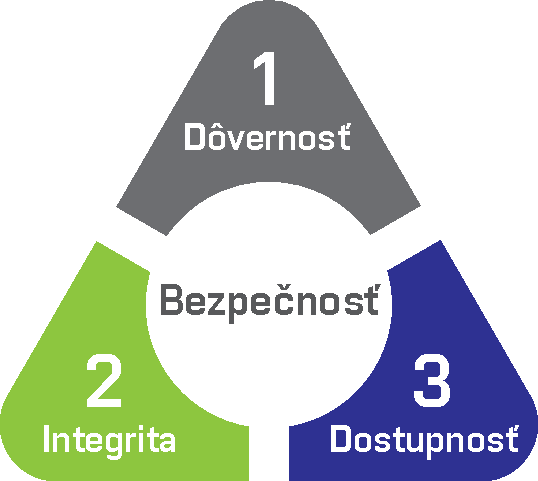
\includegraphics[scale=0.6]{obrazky/cia.pdf}
		\end{center}
		\caption[Triáda dôvernosť, integrita a dostupnosť]{Triáda dôvernosť, integrita a dostupnosť demonštrujúca potrebu všetkých troch prvkov na zaistenie bezpečnosti \cite{Vyncke2008}.}%{CIA triáda\footnotemark}				
\label{cia}
\end{figure}
%\footnotetext{Zdroj: https://www.comtact.co.uk/blog/what-is-the-cia-triad}
\end{itemize}

	\noindent
	Aj keď triáda \zk{zkCIA} definuje ciele na zaistenie bezpečnosti, tak niektorí odborníci ju nepovažujú za dostatočnú a zavádzajú ďalšie dve podmienky a pojmy  \cite{Stallings2011}:\\
	\\
	\begin{itemize}
		\item Authencity (Autenticita)\,--\,overenie originál, platnosti správy a identity jej pôvodcovi. Najčastejšie sa na zaistenie tejto podmienky využívajú certifikáty.
		\item Accountability (Sledovateľnosť)\,--\,identifikácia prístupu k~informáciám a vysledovateľnosť bezpečnostných incidentov v~prípade využitia forenznej analýzy. Väčšinou je táto požiadavka zaistená záznamom činnosti v~systéme formou logu.
	\end{itemize}





\newpage
\section{Pasívne a aktívne útoky}
Útoky na bezpečnosť môžu byť rozdelené do dvoch skupín \cite{Vyncke2008}. Jednou skupinou je pasívny útok, kde útočník nepozmeňuje pôvodné dáta a nevplýva na príjemcu týchto dát. Druhou možnosťou je aktívny útok, pri ktorom sú buď pozmenené dáta doručené príjemcovi alebo je obeť nejakým spôsobom ovplyvňovaná, napríklad zasielaním falošných informácií.

\begin{figure}[H]
	\begin{center}
		\includegraphics[scale=0.55]{obrazky/passive-attack.pdf}
	\end{center}
	\caption[Pasívny útok]{Príklad pasívneho útok, pri ktorom útočník odpočúva komunikáciu medzi dvoma uzlami \cite{Stallings2011}.}
	\label{passive-attack}
\end{figure}

Pri pasívnom útoku, ktorý je znázornený na obrázku \ref{passive-attack} ide útočníkovi prevažne o~zachytenie prenášanej komunikácie, monitorovanie a  analýzu prevádzky. Odposluch a zobrazenie obsahu dát je účinné hlavne pri nepoužití šifrovania správ medzi koncovými bodmi alebo aj pri použití slabých šifier, krátkych kľúčov a nedostatočne bezpečných hesiel. Monitorovanie prevádzky, respektíve analýza komunikácie je možná aj pri použití šifrovania, keďže každá komunikácia je charakteristická určitým vzorom. Pasívne útoky je nesmierne obtiažne detegovať nakoľko nemodifikujú dáta pri prenose. Najúčinnejšia obrana je použitie dostatočne silných šifier na zabezpečenie dát. Jeden z~pasívnych útokov sa hojne využíva aj pri prevencii v~\zkratka{zkIDS} a \zkratka{zkIPS}, kde bez analýzy prevádzky by nebolo možné zabezpečiť sieť. Pasívnymi útokmi sa nespôsobuje škoda na systéme alebo infraštruktúre, ale hrozba spočíva v~narušení dôvernosti.

\begin{figure}[H]
	\begin{center}
		\includegraphics[scale=0.55]{obrazky/active-attack-masq.pdf}
	\end{center}
	\caption[Aktívny útok maškaráda]{Príklad aktívneho útoku maškarádou, kedy uzol Eva obdrží falošnú správu od útočníka mysliac si, že ide o~správu od uzla Bob \cite{Stallings2011}.}
	\label{active-attack-masq}
\end{figure}

\begin{figure}[H]
	\begin{center}
		\includegraphics[scale=0.55]{obrazky/active-attack-dos.pdf}
	\end{center}
	\caption[Aktívny útok DOS]{Príklad aktívneho útoku DOS, pri ktorom je uzol Eva zahltený nevyžiadanými správami (označené červeno) \cite{Stallings2011}.}
	\label{active-attack-dos}
\end{figure}

\begin{figure}[H]
	\begin{center}
		\includegraphics[scale=0.55]{obrazky/active-attack-mod.pdf}
	\end{center}
	\caption[Aktívny útok modifikácia správy]{Príklad aktívneho útoku modifikáciou správy, pri ktorom je originálna správa presmerovaná cez útočníka, následne pozmenená a prijatá uzlom Eva, ktorý ju považuje za legitímnu \cite{Stallings2011}.}
	\label{active-attack-mod}	
\end{figure}

\begin{figure}[H]
	\begin{center}
		\includegraphics[scale=0.55]{obrazky/active-attack-reply.pdf}
	\end{center}
	\caption[Aktívny útok prehratím]{Príklad aktívneho útoku prehratím, pri ktorom príde uzlu Eva legitímna správa (označená modro) a následne po určitom čase aj odchytená správa od útočníka, ktorá je pozmenená (označená červeno) \cite{Stallings2011}.}
	\label{active-attack-reply}
\end{figure}

%TODO AMPLIFIKACNY UTOK, REFLEXIVNY UTOK

Aktívne útoky sú sofistikovanejšie ako pasívne, modifikujú dáta alebo vytvárajú falošné, o~ktorých prijímateľ predpokladá, že prišli od zdroja, s~ktorým pôvodne komunikoval. Hrozby, ktoré môžu týmito útokmi nastať sú strata integrity, teda modifikácia dát a ohrozenie dostupnosti pričom vždy dochádza ku škode na systéme alebo infraštruktúre. Maškaráda je prvým z~aktívnych útokov, kde ako je možné vidieť na obrázku \ref{active-attack-masq}, útočník vytvára falošnú správu, ktorú zasiela obeti a tá sa domnieva, že komunikuje s~pôvodným zdrojom, v~našom prípade Bobom. Použitím osobných certifikátov na oboch stranách by bolo možné odhaliť, že správa nepochádza od zdroja, ale od útočníka. Príkladom aktívneho útoku je aj útok odoprenia služby \ref{active-attack-dos}, kde sa vytvárajú falošné dáta generované vysokou frekvenciou (v~obrázku značené červenou farbou), za účelom odstaviť systém alebo infraštruktúru, ktorá nezvláda spracovanie toľkých požiadaviek, keďže nebola na takúto záťaž dimenzovaná. Tretím aktívnym útokom \ref{active-attack-mod} je modifikácia správy útočníkom pri prechode komunikačným kanálom, ktorý sa realizuje rôznymi technikami podvrhnutia zdroja alebo identity. Komunikácia v~tomto prípade prebieha cez útočníka, ktorý tento útok mohol uskutočniť napríklad podvrhnutím smerovania. Posledným útokom je útok prehratím \ref{active-attack-reply}, čo je útok veľmi podobný predchádzajúcemu, akurát obeť obdrží najprv pôvodnú nepozmenenú správu a následne po určitom čase aj modifikovanú správu od útočníka. Takéto správy môžu byť generované aj ako nežiadúca sieťová prevádzka pri zahltení prvkov alebo pri zlom nastavení smerovania. Citlivé sú najmä transakčné systémy napríklad databáze. Zabrániť tomuto útoku je možné pomocou časových pečiatok a jednoznačných identifikátorov. 






%% Vložení souboru 'text/bezpecnostny-audit.tex' s úvodem
\chapter{Bezpečnostný audit}
\phantomsection
\addcontentsline{toc}{chapter}{Bezpečnostný audit}

\section{Manažment rizík}
Manažment rizík je proces pozostávajúci z analýzy rizík a riadenia rizík\cite{McMillan2018}. Dôležitým faktom je, že riziko nie je možné eliminovať, ale ho iba znížiť.

Pri analýze rizík zisťujeme, aké riziká existujú, ako medzi sebou súvisia a aké škody môžu spôsobiť. Analýza rizík môže byť vykonávaná kvalitatívne a kvantitatívne.\\ 
\noindent
Štandard NIST SP 800-30\cite{7TVhmfuQFbsOANAz} definuje nasledujúce kroky pri analýze rizík:

\begin{enumerate}
	\item Identifikácia informačných aktív a ich význam
	\item Identifikácia hrozieb
	\item Identifikácia zraniteľností
	\item Zistenie pravdepodobnosti
	\item Identifikovanie dopadu
	\item Definovanie rizika ako súčinu pravdepodobnosti a dopadu
\end{enumerate} 
\vspace{2em}
Riadenie rizík má za úlohu minimalizáciu potenciálnych škôd odhalených pri analýze rizík s ohľadom na vyváženie nákladov na riadenie rizika. 
\\\\
\noindent
Prístupy k nájdenému riziku\cite{Vyncke2008}\cite{McMillan2018}:
\begin{itemize}
	\item Zníženie\,--\,aplikovanie protiopatrenia na odstránenie hrozby alebo zraniteľnosti prípadne zníženie pravdepodobnosti rizika. Nikdy nie je však možné riziko eliminovať.
	
	\item Akceptovanie\,--\,v prípade neexistujúceho protiopatrenia alebo veľmi nízkeho rizika
	
	\item Presun\,--\,riziko je možné presunúť na inú organizáciu, napr. poistenie v prípade škody spôsobenej nedostatočným zabezpečením.
	
	\item Ignorácia\,--\,úplné vypustenie faktu, že dochádza k riziku, tento prístup sa považuje za iracionálny.
\end{itemize}
\vspace{2em}
\noindent
Na ohodnotenie rizika slúžia rôzne systémy hodnotenia, jedným z nich je  \zkratka{zkCVSS}, ktorý definuje riziká podľa definovaných metrík na základe dosiahnutého skóre do nasledujúcich tried:

\begin{itemize}
	\item 0: No issue
	\item 0,1\,--\,3,9: Low
	\item 4,0\,--\,6,9: Medium
	\item 7,0\,--\,8,9: High
	\item 9,0\,--\,10,0: Critical
\end{itemize} 

%% Vložení souboru 'text/bezpecnostne-a-prevadzkove-problemy.tex' s úvodem
\chapter{Prevádzka a bezpečnosť sietí}
\phantomsection
%TODO MOZNO NIECO O PREVADZKE SIETI + BEZPECNOSTNY ASPEKT
Prevádzka sieťových zariadení je proces nielen o monitorovaní incidentov, zabezpečovaní konzistencie a konvergencie siete, ale aj o aktualizáciách softvéru a hardvéru, aplikovaní bezpečnostných zásad a politík. Táto kapitola preto opisuje jednotlivé aspekty s ktorými sa pri prevádzke siete môžeme stretnúť.

\section{Sieťové prvky}
Medzi základné stavebné piliere sietí, bez ktorých nie je možná komunikácia koncových staníc patria smerovače (router) a prepínače (switch). Mimo týchto dvoch základných zariadení sa v \zkratka{zkLAN} sieťach často vyskytujú prístupové body (access point), firewally, sieťové mosty (bridge) a v dnes už ojedinelých prípadoch ešte aj rozbočovače (hub). V súčasnosti však jedno zariadenie môže kombinovať funkcie zariadení, ktoré majú podľa modelov TCP/IP alebo ISO/OSI na starosti inú vrstvu modelu. Preto sa dnes hlavne z finančných dôvodov používajú takzvané L3 prepínače, ktoré s určitými obmedzeniami vedia nahradiť nákladné smerovače. Taktiež smerovače ako aj L3 prepínače umožňujú filtrovanie paketov, takže vedia čiastočne zastať aj základné funkcie firewallu. Značky najpoužívanejších sieťových zariadení su vyobrazené na obrázku \ref{net-devices} a budú používané v nasledujúcich kapitolách.

\begin{figure}[H]
	\begin{center}
		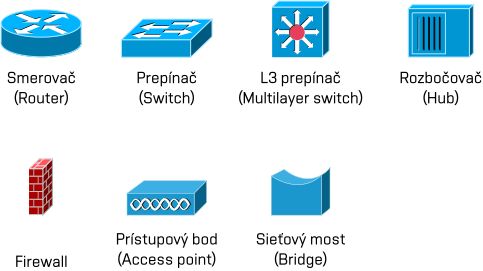
\includegraphics[scale=0.4]{obrazky/net_devices.pdf}
	\end{center}
	\vspace{-5em}
	\caption[Typy sieťových zariadení v lokálnych sieťach]{Typy sieťových zariadení v lokálnych sieťach}
	\label{net-devices}
\end{figure} 

\section{Hierarchický model sietí}
%TODO EDGE
S postupným nárastom sieťových zariadení a komplexnosti siete dochádza v sieťach bez hierarchie k mnohým problémom ako veľké broadcast domény, vysoká cena za port, vysoké zaťaženia zariadení, neprítomnosť redundancie. Preto sa zaviedol hierarchický model siete, ktorý rieši problémy veľkosti a rozsahu broadcast a kolíznych domén, umožňuje efektívne prideľovanie \zkratka{zkIP} adries a oddeľuje zariadenia pracujúce na jednotlivých vrstvách ISO/OSI.  
\\\\
\noindent
Siete sú spravidla delené do 3 vrstiev s definovanými funkciami \cite{Lammle2013}:
\begin{itemize}
	\item Core\,--\,tvorí vysokorýchlostnú chrbticu siete, agreguje dáta z distribučnej vrstvy a mala by byť redundantná. Nároky na rýchlosť portov a výkon zariadenia sú obzvlášť vysoké, a preto sa využívajú prevažne smerovače, ale taktiež ako v distribučnej vrstve dnes už aj L3 prepínače.
	\item Distribučná (Distribution)\,--\,agreguje dáta z prístupovej vrstvy, vytvára a oddeľuje broadcast domény, riadi smerovanie medzi \zkratka{zkVLAN} a  filtrovanie paketov. Táto vrstva kvôli zabezpečeniu dostupnosti využíva agregovanie  a redundanciu liniek. Typicky sa skladá zo smerovačov, no v dnešnej dobe hlavne z L3 prepínačov, keďže tie nie sú finančne také náročné. 
	\item Prístupová (Access)\,--\,vstupný bod do siete, ktorý riadi prístup a politiku pre koncové zariadenia, segmentuje sieť, vytvára a separuje kolízne domény. V neposlednej rade zariaďujú prístup k distribučnej vrstve. Je tvorená zariadeniami ako prepínač, rozbočovač alebo prístupový bod.
\end{itemize} 

\begin{figure}[H]
	\begin{center}
		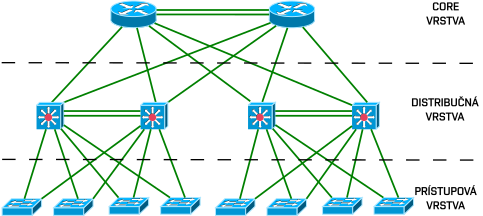
\includegraphics[scale=0.58]{obrazky/hierarchy_network.pdf}
	\end{center}
	\vspace{-11em}
	\caption[Hierarchické rozdelenie siete na vrstvy]{Hierarchické rozdelenie siete na vrstvy}
	\label{net-devices}
\end{figure} 

\noindent
\vspace{2em}
V menších sieťach prevažne malých firiem sa využíva zlučovanie vrstiev nazývaných ako collapsed core, ktoré zlučujú distribučnú a core vrstvu, prípadne zlučujú všetky tri vrstvy dokopy. 

Cieľom hierarchického modelu a dobre navrhnutej siete je dosiahnutie nasledujúcich vlastností:

\begin{itemize}
	\item Škálovateľnosť\,--\,jednoduché a bezproblémové pridanie zariadenia pri raste a rozširovaní siete.
	\item Redundancia\,--\,zabezpečenie vysokej dostupnosti viacnásobnými linkami medzi zariadeniami a zálohovanie samotných zariadení ich redundanciou.
	\item Výkonnosť\,--\,agregovanie liniek a výber dostatočne výkonných zariadení
	\item Bezpečnosť\,--\,zabezpečenie siete na viacerých úrovniach ako napríklad portoch, oddelením segmentov pomocou VLAN, riadením prístupu, šifrovaním a pod.
	\item Manažovateľnosť\,--\,vytvorenie šablón, definovaných štandardov a pravidiel na zaistenie konzistentnosti konfigurácií zariadení na jednoduchšie odhaľovanie chýb. 
	\item Udržovateľnosť\,--\,schopnosť systému prechádzať zmenami komponentov, služieb a vlastností.
\end{itemize}



\section{Úrovne sieťových prvkov}
Sieťové prvky sú zodpovedné nielen za preposielanie dát medzi koncovými stanicami, ale aj za mnohé riadiace dáta medzi sebou, bez ktorých by sieť nebola funkčná. Preto sa jednotlivé protokoly a služby rozdeľujú troch rovín alebo úrovní, a to management, control a data plane. Tieto pojmy sa využívajú vo väčšej miere v softvérovo definovaných sieťach, no sú platné aj v klasickej koncepcii.
 
Úroveň management plane je zodpovedná za konfiguráciu zariadení a riadenie prístupu ku konfiguráciám. Typickými príkladmi protokolov pracujúcich na tejto úrovni sú \zkratka{zkSNMP}, \zkratka{zkAAA}, Syslog, \zkratka{zkSSH} a mnohé ďalšie \cite{Singh2018}. Druhá úroveň, control plane má na starosti prevažne smerovanie, teda kadiaľ budú pakety smerované a prenáša riadiace a signalizačné informácie pre protokoly ako napríklad, \zkratka{zkOSPF}, Spanning tree, \zk{zkFHRP} \cite{Singh2018}. Poslednou úrovňou je data plane nazývaná často aj forwarding plane, ktorá prepína pakety na daný port na základe rozhodnutie z control plane. Táto časť sieťových prvkov musí byť veľmi rýchla, aby zaistila nízku odozvu a dostatočne vysoké prenosové rýchlosti. Nižšie uvedený obrázok \ref{sdn-planes} reflektuje tok dát z jednej úrovne do druhej a tiež medzi dvoma susednými zariadeniami. Úroveň management plane zodpovedná za konfiguráciu zariadenia a nastavuje úroveň control plane, v tomto prípade smerovanie z zariadení. Po výmene informácií so susednými smerovačmi sa vytvoria príslušné tabuľky a nakoniec smerovacia tabuľka, ktorá sa využíva pri rozhodovaní prepínania paketov v úrovni data plane.

\begin{figure}[H]
	\begin{center}
		\includegraphics[scale=0.6]{obrazky/SDN_planes.pdf}
	\end{center}
	\caption[Rozdelenie úrovní v smerovači, tok informácií v jeho vnútri a medzi susednými smerovačmi]{Rozdelenie úrovní v smerovači, tok informácií v jeho vnútri a medzi susednými smerovačmi \cite{Pepelnjak2013}}
	\label{sdn-planes}
\end{figure} 


%TODO 3 za tried source interfaces


\section{Riadenie a zneužitie prístup}
AAA, username, accounts, enable psswd, ssh, ACL(data plane, je to data plane?) 92, 111, 112, bannery plus logovanie neuspesnych pristupov

\section{Smerovacie protokoly}
autentizacia, passive, ip source routing, urpf


\section{Identifikácia zariadení, pravidiel a nastavení}
host,domainname, acl remark, int description, vlan description

\section{Šifrovanie hesiel}

\section{Logovanie}
syslog, snmp nastavenie oboch, plus co logovat, teda accouting a logovanie deny pravidiel, 93

\section{Synchronizácia času}
ntp + amplifikacne utoky

\section{Záloha a zabezpečenie konfigurácií}
archive, tftp, scp, delete protection, logovanie zmien, mozno netreba, ak je AAA accounting
\section{Správanie pri vysokom zaťažení}
68-71, storm control
\section{Monitorovanie výkonu siete}
SPAN NETFLOW
\section{Problémy vrstvy L2}
access, max, hopping, double tagging, blackhole, default access a trunk, dtp, spanning tree, dot1x, vtp
\section{First Hop Security}
130 - 138 140 144-148 aj mac spoof a mac floof, teda spanning tree prikazy!!!
http://isp-servis.com/?p=191
\section{First Hop Redundancy Protocols}

\section{Tunely}
\section{Mapovanie siete a objavovanie zariadení}
proxy arp, 88-91, lldp, cdp, 139
\section{Nepoužívané a nebezpečné služby}
\section{Ostatné}
source interfaces
loopback
shutdown 

%% Vložení souboru 'text/navrh.tex' s úvodem
\chapter{Návrh}
\phantomsection

\section{Požiadavky na aplikáciu}


O kĺúčových vlastnostiach, pridaj este zmienku o kontrole aktualnej verzie. Cisco ma API na to

\section{Existujúce riešenia a odlišnosti}

\section{Rozdelenie príkazov}
Na zariadeniach od firmy Cisco s operačným systémom IOS bol vykonaný rozbor možných príkazov a ich foriem zápisu a početnosti výskytu v konfigurácií. Tento rozbor bol spravený z dôvodu, že niektoré príkazy sa môžu opakovať a zároveň jeden druh príkazu môže byť konfigurovaný v rôznych kontextoch a teda neprítomnosť v jednom kontexte automaticky neznamená nedostatok v konfigurácií. Na základe rozboru boli rozdelené príkazy na konfiguráciu sieťových zariadení do nasledujúcich štyroch kategórií:
\\
\begin{enumerate}
	\item Maximálne s jedným výskytom v konfigurácii\,--\,príkladom môže byť verzia protokolu \zk{zkSSH}.
	
\begin{minipage}{\linewidth}		
\begin{lstlisting}[frame=single,numbers=right,caption={Konfigurácia verzie protokolu SSH},label=lst:ver-ssh,basicstyle=\ttfamily\small, keywordstyle=\color{black}\bfseries\underbar,language=,]
Router(config)#ssh version 2
\end{lstlisting}
\end{minipage}
	
	\item \vspace{2em} Viacnásobný výskyt viazaný na rozhranie\,--\,typickým príkladom je zabezpečenie portu s definovaním maximálneho počtu povolených \zkratka{zkMAC} adries.
	
\begin{minipage}{\linewidth}		
\begin{lstlisting}[frame=single,numbers=right,caption={Konfigurácia maximálneho počtu povolených MAC adries na porte},label=lst:ver-ssh,basicstyle=\ttfamily\small, keywordstyle=\color{black}\bfseries\underbar,language=,breaklines=true]
Router(config)#interface FastEthernet0/1
Router(config-if)#switchport port-security mac address maximum 1
\end{lstlisting}
\end{minipage}

	\item \vspace{2em} Viacnásobný výskyt v konfigurácii\,--\,tieto príkazy konfigurujú rôzne služby, napríklad autentizáciu správ \zkratka{zkOSPF}.

\begin{minipage}{\linewidth}		
\begin{lstlisting}[frame=single,numbers=right,caption={Konfigurácia autentizácie OSPF na porte alebo v proccese},label=lst:ver-ssh,basicstyle=\ttfamily\small, keywordstyle=\color{black}\bfseries\underbar,language=,breaklines=true]
Router(config)#interface FastEthernet0/1
Router(config-if)#ip ospf message-digest-key 1 md5 heslo
Router(config-if)#ip ospf authentication message-digest

Router(config)#router ospf 1
Router(config)#area 0 authentication message-digest
Router(config)#area 0 authentication key-chain 1
\end{lstlisting}
\end{minipage}
	
	
	\item \vspace{2em} Všeobecný príkaz pre celé zariadenie a zároveň viacnásobný výskyt viazaný na rozhranie\,--\,s týmto nastavením je možné sa stretnúť pri protokole \zkratka{zkLLDP}, ktorý je možné zapnúť pre všetky porty globálne a následne selektovať porty, na ktorých nebude bežať.
	
\begin{minipage}{\linewidth}		
\begin{lstlisting}[frame=single,numbers=right,caption={Konfigurácia protokolu LLDP a vypnutie protokolu pre jeden port},label=lst:ver-ssh,basicstyle=\ttfamily\small, keywordstyle=\color{black}\bfseries\underbar,language=,breaklines=true]
Router(config)#lldp run
Router(config)#interface FastEthernet0/1
Router(config-if)#no lldp receive
Router(config-if)#no lldp transmit
		

\end{lstlisting}
\end{minipage}
	
\end{enumerate}

\section{Rozdelenie sieťových prvkov}
Sieť je dnes navrhovaná zväčša podľa hierarchického modelu opísaného v kapitole \ref{hierarchicky-model}. Preto sa aj problémy a útoky v návrhu zatrieďujú podľa vrstvy, ktorú ovplyvňujú. V praxi sa však v menších sieťach funkcie jednotlivých vrstiev zlučujú, a preto boli okrem štandardných vrstiev nad rámec hierarchického modelu definované nasledujúce:

\begin{itemize}
	\item CORE/EDGE\,--\,core vrstva, prípadne s funkciou hraničného prvku.
	\item DIST\,--\,distribučná vrstva.
	\item ACC\,--\,prístupová vrstva.
	\item COLALL\,--\,všetky vyššie zmienené vrstvy zlúčené do jednej.
	\item COLDISTACC\,--\,zlúčená distribučná a prístupová vrstva.
	\item COLCOREDIST\,--\,zlúčená core a distribučná vrstva.
\end{itemize}


\section{Zoznam odporúčaní}
 TODO: citacie k jednotlivym riadkom, prejst este raz planes a severity, eliminovat viac riadkov s loopback, skratky z tabulky treba vypisat                                                                                                                                                                                                                                                                                                                                                                                                                                                                                                                                                                                                     

V súčasnej dobe existuje mnoho odporúčaní, štandardov a benchmarkov, ktoré sa zaoberajú bezpečnosťou a správnou konfiguráciou sieťových zariadení. V mnohých prípadoch sú buď príliš všeobecné a teda sieťoví inžinieri majú problém zistiť, čo daným odporúčaním autor myslel a ako ho implementovať, alebo sú určené iba pre zariadenia od jedného výrobcu. Problémom je taktiež, že väčšina odporúčaní, štandardov a benchmarkov sa nie úplne prekrývajú, a teda je potrebné pri nastavovaní a audite zariadení čerpať s mnohých naraz. Výsledná tabuľka obsahuje odporúčania z odbornej literatúry a štandardov a benchmarkov verejne dostupných a používaných v produkčnom nasadení. Výhodou je aj fakt, že obsahuje odporúčania vychádzajúce z problémov IPv6, ktoré nie sú často v štandardoch a benchmarkoch dostupné. Podrobná tabuľka s mapovaním odporúčaní na príkazy pre zariadenia Cisco s operačným systémom IOS je v prílohe TODO priloha %TODO priloha.

Zariadenia Cisco boli pre túto prácu vybrané z dôvodu, že spoločnosť Cisco je lídrom ktorý udáva trend, ich zariadenia sú celosvetovo v korporáciách veľmi rozšírené a mnoho literatúry a benchmarkov sa odvoláva na nastavenia týchto prístrojov s udávanými príkladmi konfigurácie. Taktiež sú tieto zariadenia dobrým referenčným príkladom pre hľadanie alternatívy v zariadeniach od iných výrobcov.

V tabuľke \ref{checklist} je možné vidieť, že odporúčania sú rozdelené podľa viacerých kritérií. V prvom rade sú to roviny (plane), ktoré nie sú dôležité pre následnú automatickú konfiguráciu a odhaľovanie problémov, ale na vytvorenie si obrazu, ktorá časť rovín je kritická a postihnuteľná najviac. 

Stĺpec závažnosť (severity) vznikol odhadom na základe znalostí a skúseností. Tento atribút bude možné zmeniť v konfiguračnom súbore každého modulu v závislosti na riziku, ktoré sa pre danú topológiu a firmu vyhodnotí za pomoci manažmentu rizík opísaného v kapitole \ref{bezpecnostny-audit}. Tento atribút sa nenachádza v žiadnom štandarde ani benchmarku, z ktorého vytvorený zoznam odporúčaní čerpal, no je veľmi dôležitý z hľadiska, že nie všetky nedostatky sú rovnako závažné a nemajú rovnaký dopad. Hodnoty, ktoré nadobúda sú prebrané zo štandardu \zk{zkCVSS}, pričom posledný interval \texttt{none} reprezentujúci nulové riziko respektíve závažnosť je zamenený za kľúčové slovo \texttt{notify}. K tejto zmene prišlo z dôvodu, že problémy s nulovým rizikom nie sú súčasťou návrhu a nemá zmysel ich riešiť. V prípade, že bude nález falošne pozitívny alebo riziko bude akceptované, tak sa táto skutočnosť uloží do konfiguračného súboru. Závažnosť \texttt{notify} bude použitá v prípade prítomnosti monitorovania portu pomocou zrkadlenia portu alebo NetFlow/sFlow. Jedná sa totiž o technológie potrebné na monitorovanie prevádzky z legislatívnych alebo bezpečnostných dôvodov. Riziko existuje iba pri nesprávnom nastavení zdrojov monitorovania a cieľu pre zber dát, a preto je dobré vedieť pri audite o prítomnosti tohto nastavenia.
 

Ďalším atribútom tabuľky je stĺpec zariadenie (facility), ktorý rozlišuje ktorých zariadení sa problém alebo útok týka. Zariadenia sú rozdelené na smerovač (R), prepínač (L2SW) a L3 prepínač (L3SW). Rozdelenie na prvky z L2 a L3 vrstvy môže byť vykonané automaticky na základe rozpoznania v konfigurácií.

Posledným rozdelením je vrstva, na ktorej zariadenie pracuje (facility layer), nakoľko rozdelenie podľa zariadení nie je dostatočné, pretože napríklad L3 prepínač môže byť použitý na ktorejkoľvek vrstve hierarchického modelu a každá vrstva má určité špecifiká, ktoré neobsahuje iná vrstva. Každý konfiguračný súbor popisujúci zariadenie bude obsahovať informáciu, do ktorej vrstvy patrí a na základe toho bude môcť program rozhodnúť, ktoré moduly zodpovedné za nájdenie problému a jeho vyriešenie budú na zariadení spustené. Taktiež bude možné meniť, dopĺňať a zakázať spúšťanie modulov pre jednotlivé zariadenia, pokiaľ by v danej topológii nevyhovovalo rozdelenie z tabuľky \ref{checklist}. 

Vrstva, na ktorej zariadenie operuje, ako aj definované zariadenie, ktorého sa odporúčanie a opatrenie týka nie sú súčasťou žiadneho kontrolného zoznamu, benchmarku ani štandardu, z ktorého bolo čerpané. Sieťový administrátor preto musí sám vyvodiť záver, ktoré odporúčania a postupy bude aplikovať na jednotlivé zariadenia a vrstvy hierarchického modelu. Preto vytvorená tabuľka odporúčaní už obsahuje aj zoznam zariadení, ktorých sa opatrenie týka.


\scriptsize
\begin{longtable}{|P{8em}|P{9em}|P{8em}|P{5em}|P{5em}|P{10em}|}
	\captionsetup{font=normalsize}
    \hline
    Útok / Problém & Mitigácia / Konfigurácia typu “Best practise” & Plane \hspace{2em}{[}DATA| CONTROL| \hbox{MANAGEMENT}{]} & Severity {[}\hbox{CRITICAL}| HIGH| MEDIUM| LOW| NOTIFY{]}\cite{McMillan2018} & Facility\hspace{1em}{[}R| L3SW| L2SW{]} & Facility layer \hspace{2em} {[}ACC| DIST| \hbox{CORE/EDGE}| COLALL| \hbox{COLDISTACC}| \hbox{COLCOREDIST}{]} \\ \hline
    \endhead
    %
    Nepovolený prístup k manažovaniu zariadenia & Vytvoriť a aplikovať ACL pre OOB, Telnet, SSH a pod. a zaznamenať v logu prístupy & Management & CRITICAL & VŠETKY & VŠETKY \\ \hline
    Nemožná identifikácia zariadenia & Vytvoriť hostname & Management & LOW & VŠETKY & VŠETKY \\ \hline
    Nemožnosť vzdialeného prístupu & Vytvoriť doménové meno & Management & LOW & VŠETKY & VŠETKY \\ \hline
    Neautorizovaný prístup cez nepoužívané a nezabezpečené protokoly na manažment zariadení & Vypnúť nepoužívané protokoly na prístup k manažovaniu zariadení (telnet a pod.) & Management & HIGH & VŠETKY & VŠETKY \\ \hline
    Prítup bez požadovaných prístupových údajov & Nakonfigruovanie protokolov na manažment zariadení, aby požadovali prístupové údaje (telnet a pod.) & Management & CRITICAL & VŠETKY & VŠETKY \\ \hline
    Nepoužívanie zabezpečeného protokolu na manažment zariadení môže viesť k odposluchu & Zapnutie SSH & Management & CRITICAL & VŠETKY & VŠETKY \\ \hline
    Nebezpečná verzia 1 protokolu SSH & SSH verzia 2 & Management & CRITICAL & VŠETKY & VŠETKY \\ \hline
    Útok na krátky RSA kĺúč & Dĺžka RSA kľúča minimálne 2048 bitov & Management & CRITICAL & VŠETKY & VŠETKY \\ \hline
    Dlhé neaktívne sedenie môže byť zneužité alebo aj fyzický prístup útočníka k aktívnemu sedeniu môže viesť k zmene konfigurácie & SSH čas vypršania sedenia & Management & MEDIUM & VŠETKY & VŠETKY \\ \hline
    Hádanie hesla k RSA kľúču & SSH maximálny počet neúspešných pokusov & Management & HIGH & VŠETKY & VŠETKY \\ \hline
    Útok hrubou silou na zistenie prihlasovacích údajov & Špecifikovať čas po ktorý nie je možné po N pokusoch sa prihlásiť & Management & HIGH & VŠETKY & VŠETKY \\ \hline
    Prihlásenie na zariadenie nie je možné kvôli zablokovaniu pre príliš veľa neúspešných pokusov & Povolenie prístupu administrátorovi na základe IP adresy, keď je protokol na manažovanie zariadení nedostupný kvôli DOS útoku & Management & MEDIUM & VŠETKY & VŠETKY \\ \hline
    Dlhé neaktívne sedenie môže byť zneužité alebo aj fyzický prístup útočníka k aktívnneum sedeniu môže viesť k zmene konfigurácie & Čas vypršania sedenia pre protokol na manažovanie zariadení & Management & MEDIUM & VŠETKY & VŠETKY \\ \hline
    Možné prihlásenie do zariadenia cez telnet keď je prítomné SSH & Zakázať telnet ak je SSH aktívne & Management & CRITICAL & VŠETKY & VŠETKY \\ \hline
    Útočník nie je informovaný o právnych následkoch & Právne upozornenie pri prístupe k zariadeniu & Management & LOW & VŠETKY & VŠETKY \\ \hline
    Možnosť prečítať heslá z uniknutých konfigurácií & Zašifrovanie hesiel v otvorenej podobe & Management & CRITICAL & VŠETKY & VŠETKY \\ \hline
    Nepovolená zmena konfigurácie zariadenia & Vytvorenie hesla na editovanie konfigurácie zariadenia & Management & CRITICAL & VŠETKY & VŠETKY \\ \hline
    Nepovolený prístup k manažmentu konfigurácie zariadenia & Lokálne zabezpečené účty & Management & CRITICAL & VŠETKY & VŠETKY \\ \hline
    Centrálna správa prihlásení a dohľadateľnosť zmien v konfigurácií & Definovanie a povolenie AAA serveru na prihlásenie a definovanie záložného prihlásenia & Management & HIGH & VŠETKY & VŠETKY \\ \hline
    Centrálna správa prihlásení a dohľadateľnosť zmien v konfigurácií & Definovanie a povolenie AAA serveru na editáciu konfigurácií a definovanie záložného prihlásenia & Management & MEDIUM & VŠETKY & VŠETKY \\ \hline
    Hádanie prístupových údajov & Definovanie maximálneho počtu neúspešných pokusov o prihlásenie a následné zablokovanie účtu & Management & HIGH & VŠETKY & VŠETKY \\ \hline
    Prihlásenie bez prihlasovacích údajov & Zakázať záložné prihlásenie bez poskynutia autentizačných prostriedkov & Management & CRITICAL & VŠETKY & VŠETKY \\ \hline
    AAA používa primárne lokálne účty namiesto centralizovaných na serveri & AAA nesmie používať ako prvú možnosť prihlásenia lokálny účet & Management & HIGH & VŠETKY & VŠETKY \\ \hline
    Používateľ prihlásený do zariadenia môže spúšťať akékoľvek príkazy & Nastavenie AAA autorizácie pre spúštanie príkazov. V prípade výpadku AAA serveru, bude užívateľ odhlásený a následne prihlásený podľa  záložného prihlásenia, aby mu nebolo pridelené vysoké oprávnenie umožňujúce vykonávať príkazy, na ktoré nemá právo & Management & HIGH & VŠETKY & VŠETKY \\ \hline
    Administrátor vloží zlý príkaz a po čase je ho nemožné dohľadať a zjednať nápravu & Nastavenie AAA účtovania respektíve logovania pripojení a vykonaných príkazov & Management & HIGH & VŠETKY & VŠETKY \\ \hline
    AAA zdrojové rozhranie nie je rovnaké pri každom reštarte & Definovanie loopback zdrojového rozhrania pre AAA & Management & MEDIUM & VŠETKY & VŠETKY \\ \hline
    Odpočúvanie SNMP verzie 1 a 2c & Použitie SNMP verie 3 pokiaľ je SNMP používané & Management & CRITICAL & VŠETKY & VŠETKY \\ \hline
    Modifikovanie konffigurácie pomocou SNMP & Obmedzenie SNMP iba na čítanie & Management & CRITICAL & VŠETKY & VŠETKY \\ \hline
    Neoprávnený prístup k SNMP informáciám & Obmedzenie SNMP iba pre vybrané IP adresy & Management & HIGH & VŠETKY & VŠETKY \\ \hline
    Administrátor nemá povedomie o problémoch na zariadení & Povolenie asynchrónnych správ SNMP TRAP & Management & MEDIUM & VŠETKY & VŠETKY \\ \hline
    Odpočúvanie SNMP sedenie z dôvodu slabého šifrovania a hashovacej  funkcie & Vytvorenie SNMP verzie 3 užívateľa s minimálnym šifrovaním AES 128 bit a hashovacou funkciou SHA & Management & CRITICAL & VŠETKY & VŠETKY \\ \hline
    Sťažená identifikácia SNMP správ z rôznych IP & Definovanie lokácie SNMP serveru & Management & LOW & VŠETKY & VŠETKY \\ \hline
    SNMP zdrojové rozhranie nie je rovnaké pri každom reštarte & Definovanie loopback zdrojového rozhrania pre SNMP & Management & MEDIUM & VŠETKY & VŠETKY \\ \hline
    Zmeny názvov rozhraní medzi reštartami a nemožnosť monitorovanie pomocou SNMP & SNMP statické nemenné meno rozhrania aj po reštarte zariadenia & Management & HIGH & VŠETKY & VŠETKY \\ \hline
    Administrátor nemá povedomie o problémoch na zariadení & Povolenie logovania protokolom SYSLOG a špecifikovanie IP adresy SYSLOG serveru & Management & HIGH & VŠETKY & VŠETKY \\ \hline
    Neprijímanie všetkých dôležitých incidentov na zariadení z protokolu SYSLOG & Špecifikovanie dôležitosti oznámenií SYSLOG na INFORMATIONAL & Management & MEDIUM & VŠETKY & VŠETKY \\ \hline
    SYSLOG zdrojové rozhranie nie je rovnaké pri každom reštarte & Definovanie loopback zdrojového rozhrania pre \hbox{SYSLOG} & Management & MEDIUM & VŠETKY & VŠETKY \\ \hline
    Nedostatočné a neštandardné formáty času v logovacích správach & Definovanie formátu času pre logovacie a ladiace výstupy & Management & MEDIUM & VŠETKY & VŠETKY \\ \hline
    Administrátor nevidí dôležité incidenty pri prihlásení a konfigurovaní cez konzolu & Vypisovanie \hbox{SYSLOG} správ \hbox{CRITICAL} a dôležitejších do terminálu & Management & MEDIUM & VŠETKY & VŠETKY \\ \hline
    Malá vyrovnávacia pamäť pre SYSLOG je dôvodom zahadzovanie správ & Definovanie veľkosti SYSLOG buffera dôležitosti oznámení na INFORMATIONAL & Management & HIGH & VŠETKY & VŠETKY \\ \hline
    Neprístupný SYSLOG server spôsobuje zahadzovanie dôležitých syslog správ & Definovanie dočasného úložiska SYSLOG správ v prípade nedostupnosti servera & Management & HIGH & VŠETKY & VŠETKY \\ \hline
    Skenovanie a zistenie informácií o sieti za pomoci protokolu CDP a využitie bezpečnostných chýb & Zakázanie protokolu CDP & Management & CRITICAL & VŠETKY & VŠETKY \\ \hline
    Skenovanie a zistenie informácií o sieti za pomoci protokolu LLDP a využitie bezpečnostných chýb & Zakázanie protokolu LLDP & Management & CRITICAL & VŠETKY & VŠETKY \\ \hline
    Nekonzistencia časov v logoch a problém pričlenenia logov k relevantným incidentom & Nastavenie NTP serveru pre aktuálny čas v logoch & Management & HIGH & VŠETKY & VŠETKY \\ \hline
    Pripojenie servera s rovnakou IP adresou, ale falošným časom & Nastavenie NTP autentizácie & Management & HIGH & VŠETKY & VŠETKY \\ \hline
    NTP zdrojové rozhranie nie je rovnaké pri každom reštarte & Definovanie loopback zdrojového rozhrania pre NTP & Management & MEDIUM & VŠETKY & VŠETKY \\ \hline
    Väčšia bezpečnosť (pub/priv key) NTP a podpora IPv6 & Použitie NTP verzie 4 & Management & MEDIUM & VŠETKY & VŠETKY \\ \hline
    Falošný čas od podvrhnutého NTP zdroja & Nastavenie NTP peer s inými sieťovými zariadeniami na krížovú validáciu času a záložný zdroj času & Management & MEDIUM & VŠETKY & VŠETKY \\ \hline
    Útočník s fyzickým prístupom k zariadeniu alebo portu môže odpočúvať alebo posielať škodlivý obsah & Explicitne zakázať nepoužívané porty & Data & CRITICAL & VŠETKY & VŠETKY \\ \hline
    Zdrojové rozhranie pre management a control protokoly & Vytvorť Loopback rozhranie s IP adresou & Control & MEDIUM & VŠETKY & VŠETKY \\ \hline
    Identifikácia pravidla v ACL & Popis každého pravidla v ACL pre lepšiu identifikáciu & Management & LOW & VŠETKY & VŠETKY \\ \hline
    Indentifikácia rozhrania & Popis každého rozhrania & Management & LOW & VŠETKY & VŠETKY \\ \hline
    SSH zdrojové rozhranie nie je rovnaké pri každom reštarte & Definovanie loopback zdrojového rozhrania pre SSH & Management & MEDIUM & VŠETKY & VŠETKY \\ \hline
    DOS útok na štandardný SSH port 22 & Špecifikovanie iného portu pre SSH ako štandardného alebo aplikovanie port knocking & Management & HIGH & VŠETKY & VŠETKY \\ \hline
    Nepovolený prístup k manažmentu konfigurácie zariadenia & Vypnutie odchádzajúcich spojení pre protokoly na manažment zariadení pokiaľ sa nepoužívajú (telnet a pod.) & Management & HIGH & VŠETKY & VŠETKY \\ \hline
    Odpočuvanie konfigurácií zariadení pri zálohe & Zapnutie zabezpečenej zálohy na server (SFTP, SCP) & Management & HIGH & VŠETKY & VŠETKY \\ \hline
    Vymazanie konfigurácie & Zapnutie ochrany pred výmazom konfigurácie & Management & HIGH & VŠETKY & VŠETKY \\ \hline
    Možnosť urobiť diff zmien konfigurácií a jej návrat & Periodické zálohovanie konfigurácie a logovanie jej zmien & Management & MEDIUM & VŠETKY & VŠETKY \\ \hline
    DOS útok alebo pokus o prístup k tomu, čo nie je povolené & Logovanie pravidiel zahodenia paketov v ACL & Management & MEDIUM & VŠETKY & VŠETKY \\ \hline
    Nízky stav voľnej pamäte & Nastavenie notifikácie pri dochádzaní pamäte & Management & MEDIUM & VŠETKY & VŠETKY \\ \hline
    Logovacie správy nemôžu byť zaznamenané kvôli nedostatku pamäte & Rezervovanie pamäte pre kritické notifikácie pri nedostatku pamäte & Management & HIGH & VŠETKY & VŠETKY \\ \hline
    Vysoké zaťaženie CPU & Nastavenie notifikácie vysokom zaťažení CPU & Management & MEDIUM & VŠETKY & VŠETKY \\ \hline
    Vysoké zaťaženie zariadenia spôsobilo nemožnosť prihlásenia k nemu & Rezervovanie pamäte preprotokoly na manažment zariadení pri nedostatku pamäte & Management & HIGH & VŠETKY & VŠETKY \\ \hline
    Pretečenie pamäte & Povoliť mechanizmy na detekciu pretečenia pamäte & Management & MEDIUM & VŠETKY & VŠETKY \\ \hline
    Načítanie škodlivej konfigurácie zo siete počas bootovania & Vypnutie načítania operačného systému alebo konfigurácie zo siete pokiaľ to nie je nutné & Management & MEDIUM & VŠETKY & VŠETKY \\ \hline
    Proxy ARP môže viesť k obídeniu PVLAN a rozširuje broadcast doménu & Vypnutie Proxy ARP & Control & CRITICAL & R, L3SW & CORE/EDGE, DIST, COLCOREDIST, COLDISTACC, \hbox{COLALL} \\ \hline
    DOS útok na stanicu, cez ktorú bola špecifikovaná cesta a teda nemožnosť komunikácie s koncovým bodom. Alebo zosnovanie MITM útoku & Vypnutie IP source routing & Control & CRITICAL & R, L3SW & CORE/EDGE, DIST, COLCOREDIST, COLDISTACC, \hbox{COLALL} \\ \hline
    DOS útok pomocou podvrhnutej IP adresy alebo vzdialený útok na smerovací protokol & Zapnutie reverse path forwarding strict/loose mode & Control & HIGH & R, L3SW & CORE/EDGE, DIST, COLCOREDIST, COLDISTACC, \hbox{COLALL} \\ \hline
    Nepoužívané, staré a nezabezpečené služby môžu byť použité na škodlivé účely & Vypnutie nepoužívaných služieb z bezpečnostných dôvodov a na šetrenie CPU a pamäte & Záleží na výrobcovi a zariadení & HIGH & Záleží na výrobcovi a zariadení & Záleží na výrobcovi a zariadení \\ \hline
    Útočník môže zistiť, že IP adresa, na ktorú skušal ping je nesprávna & Vypnutie spáv ICMP Unreachable & Data & HIGH & R, L3SW & CORE/EDGE, DIST, COLCOREDIST, COLDISTACC, \hbox{COLALL} \\ \hline
    Útočník môže zistiť masku podsiete pomocou ICMP Mask reply & Vypnutie spáv ICMP Mask reply & Data & HIGH & R, L3SW & CORE/EDGE, DIST, COLCOREDIST, COLDISTACC, \hbox{COLALL} \\ \hline
    Umožňuje DOS Smurf útok, mapovanie siete pomocou ping na broadcast adresu vzdialenej siete & Vypnutie ICMP echo správ na broadcast adresu, vypnutie directed broadcasts & Data & CRITICAL & R, L3SW & CORE/EDGE, DIST, COLCOREDIST, COLDISTACC, \hbox{COLALL} \\ \hline
    Útočník môže zistiť smerovacie informácie alebo vyťažiť CPU & Vypnutie spáv ICMP Redirects & Data & HIGH & R, L3SW & CORE/EDGE, DIST, COLCOREDIST, COLDISTACC, \hbox{COLALL} \\ \hline
    Nekonzistenia konfiguračných súborov pri zmenách konfigurácie viac ako jedným administrátorom & Povolit súčasne iba jednému administrátorovi vykonávanie zmien v konfigurácii & Management & HIGH & VŠETKY & VŠETKY \\ \hline
    Problém identifikácie SYSLOG správ s rovnakou časovou značkou & Pridanie sekvenčného čísla ku každej syslog správe & Management & LOW & VŠETKY & VŠETKY \\ \hline
    Nemožnosť prihlásenia pri zaseknutom TCP spojení & Terminovanie zaseknutého TCP spojenia & Management & MEDIUM & VŠETKY & VŠETKY \\ \hline
    Vloženie a manipulácia so smerovacími informáciami & Autentizácia smerovacích protokolov (nie heslá v otvorenej podobe) & Control & HIGH & R, L3SW & CORE/EDGE, DIST, COLCOREDIST, COLDISTACC, \hbox{COLALL} \\ \hline
    OSPF virtuálne linky degradujú výkon & Vypnutie virtuálnych liniek pre OSPF & Control & HIGH & R, L3SW & CORE/EDGE, DIST, COLCOREDIST, COLDISTACC, \hbox{COLALL} \\ \hline
    Koncové zariadenie, užívateľ a útočník môžu vidiet smerovacie správy a topológiu siete alebo pripojenie škodlivého zariadenia, ktoré vysielať a prijímať smerovacie správy & Špecifikovanie rozhraní, ktoré nebudú prijímať routovacie informácie & Control & HIGH & R, L3SW & CORE/EDGE, DIST, COLCOREDIST, COLDISTACC, \hbox{COLALL} \\ \hline
    Nemožnosť sprevádzkovať procesy smerovacích protokolov v určitých prípadoch pri použití IPv6 & Špecifikovanie identifikátorov smerovacích protokolov pre každý router (router ID) & Control & MEDIUM & R, L3SW & CORE/EDGE, DIST, COLCOREDIST, COLDISTACC, \hbox{COLALL} \\ \hline
    Vysledovateľnosť nefunkčnosti routovacieho protokolu a nesprávneho nastavenia & Zaznamenie zmeny v logu pri zmenách v smerovaní & Control & MEDIUM & R, L3SW & CORE/EDGE, DIST, COLCOREDIST, COLDISTACC, \hbox{COLALL} \\ \hline
    Škodlivé vloženie smerovacích informácií informácií, vzdialený útok & TTL security & Control & HIGH & R, L3SW & CORE/EDGE, DIST, COLCOREDIST, COLDISTACC, \hbox{COLALL} \\ \hline
    Nesprávne smerovanie kvôli sumarizácií & Vypnutie automatickej sumarizácie smerovacích protokolov & Control & HIGH & R, L3SW & CORE/EDGE, DIST, COLCOREDIST, COLDISTACC, \hbox{COLALL} \\ \hline
    Packety budú spracovávané v CPU, ktoré môže byť preťažené a môže byť zmenené smerovanie na obídenie bezpečnostnej kontroly & Zahadzovanie IPv4 paketov s rozšírenou hlavičkou (IP Options filtering) & Control & CRITICAL & R, L3SW & CORE/EDGE, DIST, COLCOREDIST, COLDISTACC, \hbox{COLALL} \\ \hline
    Odpočúvanie komunikácie  cez nezabezpečené tunely & Vypnúť tunely ktoré nie sú zabezpečené alebo zabezpečiť tunely & Data & CRITICAL & R, L3SW & CORE/EDGE, DIST, COLCOREDIST, COLDISTACC, \hbox{COLALL} \\ \hline
    Môže byť zneužité odpočúvanie pokiaľ sa používa monitorovanie prevádzky a monitorovanie prevádzky kvôli legislatívnym potrebám & Monitorovanie výkonnosti siete a zber sieťového prenosu kvôli legislatívnym potrebám & Control & NOTICE & VŠETKY & VŠETKY \\ \hline
    IP spoofing & Špecifikácia ACL na zakázanie a logovanie privátnych a špeciálnych IP adries z RFC 1918, RFC 3330 & Control & CRITICAL & R, L3SW & CORE/EDGE, COLCOREDIST, \hbox{COLALL} \\ \hline
    IP spoofing & Špecifikácia ACL na zakázanie a logovanie špeciálnych IPv6 adries z RFC 5156 & Control & CRITICAL & R, L3SW & CORE/EDGE, COLCOREDIST, \hbox{COLALL} \\ \hline
    Rogue root bridge & Rogue root bridge protection (root guard) & Control & CRITICAL & L3SW, L2SW & DIST, COLDISTACC, ACC \\ \hline
    Pripojenie pripínaču na koncový prístupový port & BPDU protection (BPDU guard) & Control & CRITICAL & L3SW, L2SW & DIST, COLDISTACC, ACC \\ \hline
    Rýchlosť konvergencie & Prístupové porty by sa nemali podielať na STP procese & Control & HIGH & L3SW, L2SW & DIST, COLDISTACC, ACC \\ \hline
    Unidirectional communication between switches can lead to loop topology/ Jednosmerná komunikácia medzi prepínačmi môźe viesť k topoógií so slučkami & Špeciálne konfigurácie zaisťujúce bezslučkovú topológiu pomocou STP keď nastane jednosmerná komunikácia (Loop Guard) & Control & CRITICAL & L3SW, L2SW & DIST, COLDISTACC, ACC \\ \hline
    Nemožnosť identifikácie účelu VLAN & Pridanie mena k VLAN & Control & LOW & L3SW, L2SW & DIST, COLDISTACC, ACC \\ \hline
    Špeciálna VLAN pre manažment na obmedzenie prístupu iba pre administrátorov & Vytvorenie separátnej VLAN pre manažment & Control & MEDIUM & L3SW, L2SW & DIST, COLDISTACC, ACC \\ \hline
    Útočníkovi s fyzickým prístupom k portu môže byť pridelený prístup do časti siete, ktorá zodpovedá príslušnej VLAN & Vytvorenie špeciálnej black hole VLAN pre nevyužité porty & Control & CRITICAL & L3SW, L2SW & DIST, COLDISTACC, ACC \\ \hline
    Predvolenej VLAN je povolené prepnute na akýkoľvek port, VLAN hopping, double tagging & Odobrať všetky porty z predvolenej VLAN & Control & CRITICAL & L3SW, L2SW & DIST, COLDISTACC, ACC \\ \hline
    Predvolenej VLAN je povolené byť prepnutá na akýkoľvek port, VLAN hopping, double tagging & Vytvorenie natívnej VLAN rozdielnej ako predvolená, priradeni k trunk portu a povolenie iba potrebných portov & Control & CRITICAL & L3SW, L2SW & DIST, COLDISTACC, ACC \\ \hline
    DTP útok, Switch spoofing útok & Vypnutie dynamického trunkovacieho protokolu a explicitne určiť porty ako prístupové a trunk & Control & CRITICAL & L3SW, L2SW & DIST, COLDISTACC, ACC \\ \hline
    MAC Spoofing, MAC Flooding & Definovanie maximálne 1 MAC adresy na port, priradenie MAC adresy na port & Control & CRITICAL & L3SW, L2SW & DIST, COLDISTACC, ACC \\ \hline
    MAC Spoofing, MAC Flooding & Nastavenie režimu narušenia, ktorý vypne port alebo informuje správcu o pripojení nepovoleného zariadenia & Control & HIGH & L3SW, L2SW & DIST, COLDISTACC, ACC \\ \hline
    Nový prepínač s vyšším číslom revízie, ale s nesprávnou VLAN databázou môže šíriť falošné VLAN identifikátory a spôsobiť nefunkčnosť siete, veľa možnćh VTP útokov kvǒli zraniteľnostiam & Vypnutie MVRP. MRP, GARP, VTP po úspešnej propagácií VLAN & Control & CRITICAL & L3SW, L2SW & DIST, COLDISTACC, ACC \\ \hline
    VTP musí byť používané & Use VTP v3 with set password and enable VTP prunning when VTP must be enabled/ Uprednostniť VTP verzie 3, špecifikovať skryté heslo a zapnúť VTP prunning pokiaľ musí byť VTP zapnuté & Control & CRITICAL & L3SW, L2SW & DIST, COLDISTACC, ACC \\ \hline
    Vysoké zaťaženie linky & Poslanie notifikácie pri prekročení prahovej hodnoty zaťaženia linky & Control & MEDIUM & VŠETKY & VŠETKY \\ \hline
    Využívanie siete nepovolenými používateľmi & Zapnutie 802.1x & Control & HIGH & L3SW, L2SW & DIST, COLDISTACC, ACC \\ \hline
    Útok hrubou silou hádaním prístupových údajov pre 802.1x & Limitovanie maximálneho počtu neúspešných pokusov o autentizáciu 802.1x & Control & HIGH & L3SW, L2SW & DIST, COLDISTACC, ACC \\ \hline
    IPv6 ND Spoofing & IPv6 ND Inspection & Control & CRITICAL & L3SW, L2SW & DIST, COLDISTACC, ACC \\ \hline
    Rogue RARA FloodRoute Information Option injectionRA RouterLifeTime=0 & RA Guard & Control & CRITICAL & L3SW, L2SW & DIST, COLDISTACC, ACC \\ \hline
    DHCP spoofing & DHCP snooping, IPv6 Snooping, DHCPv6 Guard & Control & CRITICAL & L3SW, L2SW & DIST, COLDISTACC, ACC \\ \hline
    Příliš veľa DHCP paketov, zaplavenie DHCP paketmi & Odmedziť počet DHCP paketov na nedôverihodných rozhraniach & Control & MEDIUM & L3SW, L2SW & DIST, COLDISTACC, ACC \\ \hline
    ARP Spoofing & Dynamic ARP Inspection & Control & CRITICAL & L3SW, L2SW & DIST, COLDISTACC, ACC \\ \hline
    IP spoofing & IPv4/IPv6 Source Guard & Control & CRITICAL & L3SW, L2SW & DIST, COLDISTACC, ACC \\ \hline
    IPv6 Next Header  a IPv6 Fragmentation útok & ACL blokujúce nerozpoznateľne rozšírené hlavičky & Control & CRITICAL & VŠETKY & VŠETKY \\ \hline
    Mapovanie sete pomocou pingu na multicast adresu všetkých uzlov a MLD Query Overload a Smurf útok & ACL blokujúce ICMP echo request na multicast adresu všetkých uzlov a MLD Query na prístupových portoch & Control & MEDIUM & L3SW, L2SW & DIST, COLDISTACC, ACC \\ \hline
    Mobilné zariadenia pripojené bezdôtovo spotrebovávajú veľa energie kvôli častým RA správam & RA Throttling & Control & LOW & L3SW, L2SW & DIST, COLDISTACC, ACC \\ \hline
    Zlyhanie zariadenia alebo linky môže viest k nefunkčnosti siete & Povolenie FHRP s autentizáciou a aktuálnou verziou & Control & MEDIUM & R, L3SW & CORE/EDGE, COLCOREDIST, \hbox{COLALL} \\ \hline
    Vyčerpanie cache susedov & Statický záznam pre kritické zariadenia (servery) spájajúce IP a MAC adresu a VLAN & Control & CRITICAL & L3SW, L2SW & DIST, COLDISTACC, ACC \\ \hline
    Vyčerpanie cache susedov & Na zabránenie vzdialeného útoku na cache susedov cez internet je potreba nastaviť ACL, kde povolujeme iba komunikáciu s cieľovými IPv6 adresami, ktoré sa nachádzajú v našej sieti & Control & CRITICAL & R, L3SW & CORE/EDGE, COLCOREDIST, \hbox{COLALL} \\ \hline
    Vyčerpanie cache susedov & IP destination Guard (First Hop Security) & Control & CRITICAL & L3SW, L2SW & DIST, COLDISTACC, ACC \\ \hline
    Vyčerpanie cache susedov & Limitovanie počtu IPv6 adries v cache susedov & Control & CRITICAL & L3SW, L2SW & DIST, COLDISTACC, ACC \\ \hline
    Vyčerpanie cache susedov & Limitovanie času IPv6 adresy v cache susedov & Control & CRITICAL & L3SW, L2SW & DIST, COLDISTACC, ACC \\ \hline
    Vyčerpanie cache susedov & Skrátenie IPv6 prefixu, aplikovateľné iba pr použití DHCPv6 & Control & CRITICAL & R, L3SW & CORE/EDGE, COLCOREDIST, \hbox{COLALL} \\ \hline
    SYN Flood & Nastavenie zachytávanie firewallom pre útok flagu SYN & Control & CRITICAL & R, L3SW & CORE/EDGE, COLCOREDIST, \hbox{COLALL} \\ \hline
    Komplexné bezpečnostné hrozby a narušenie bezpečnosti & Nastavenie IDS/IPS & Control & HIGH & R, L3SW & CORE/EDGE, COLCOREDIST, \hbox{COLALL} \\ \hline
		
	\caption{Zoznam bezpečnostných a prevádzkových problémov a odporúčaní}
	\label{checklist}\\
\end{longtable}

 
\section{Hierarchická štruktúra}
Stromová štruktúra a koncept fungovania, Možno fungovanie cez nejaký UML diagram (sekvenčný?) alebo skôr niečo zjednodušené





%% Vložení souboru 'text/implementacia.tex' s úvodem
\chapter{Implementácia}
\phantomsection

TODO\\
Rozdelenie zariadení a automatické vypĺňanie štruktúr YAML súborov\\
Matchovanie cez regexy, teória o REGEX (možno do teórie)\\



%% Vložení souboru 'text/zaver' se závěrem
\chapter*{Záver}
\phantomsection
\addcontentsline{toc}{chapter}{Záver}


%Buducnost - oznacovanie flase possive + komenty\\
%Dorobit backend - server \\
%co som mal spravit
%co som spravilk

% co sa nepodarili
% v skratke vyhody
% co bolo nutne nastudovat plus z kolko guidov som cerpal





Cieľom tejto diplomovej práce bol návrh a následná implementácia programu na nájdenie bezpečnostných a prevádzkových nedostatkov v sieťových zariadeniach, ako aj ich náprava pomocou generovania opravnej konfigurácie. Z tohto dôvodu bola naštudovaná problematika bezpečnosti a prevádzky sieťových zariadení a ich správna konfigurácia. Z množstva dostupnej literatúry, štandardov a odporúčaní bol vytvorený zoznam odporúčaní, na základe ktorého boli zostavované YAML moduly pre výsledný program. Tento zoznam odporúčaní bol rozšírený aj o hodnotenie závažnosti nedostatkov a priradenie prvkov zoznamu k relevantným zariadeniam v hierarchickom modely siete. Jedná sa teda o unikátne riešenie medzi bezplatnými zoznamami odporúčaní. Tento zoznam môže byť použitý aj na rozšírenie programu o podporu iných výrobcov, ale aj separátne bez akéhokoľvek využitia v programe. Vzhľadom na časovú náročnosť boli vytvorené moduly zatiaľ pre zariadenia značky Cisco. Bolo nutné zanalyzovať niekoľko stovák príkazov a ich povolených kombinácií, vytvoriť pre ne korešpondujúce regulárne výrazy a následne vytvoriť viac ako 230 YAML modulov zodpovedných za nájdenie problémov v konfiguráciách. 

Ako implementačný jazyk bol využitý Python 3.7, ktorý zaisťuje prenositeľnosť programu na viaceré platformy. Program na rozdiel od konkurencie umožňuje rozšírenie vďaka modularite aj na ďalších výrobcov sieťových zariadení a pridáva kontrolu aj pre topológie využívajúce IPv6. Taktiež rešpektuje hierarchický model siete, a teda generuje oveľa menej falošne pozitívnych správ, keďže kontroluje iba nastavenia typické pre danú vrstvu, na ktorej zariadenie operuje. Jeho výstupom je okrem iného aj prehľadná správa o kontrole zobraziteľná v PDF alebo vo webovom prehliadači. Naviac ako jediný z porovnávaných bezplatných riešení umožňuje automatické vygenerovanie nápravy, pokiaľ je to z charakteru príkazu možné. 

Program bol otestovaný pomocou vyexportovaných konfigurácií z viacerých testovacích topológií vytvorených v nástroji GNS3. Je však žiadúce aplikáciu otestovať komplexnejšie aj na reálnych a rozsiahlejších topológiách pre čo najlepšie vyladenie jej funkčnosti. 

Nástroj je možné vďaka modularite v budúcnosti rozšíriť aj o podporu na ďalších výrobcov ako Juniper a HP. Využiteľná by bola taktiež možnosť editovať záverečné správy pridaním back-endu pre HTML správy, teda označovaním falošne pozitívnych nálezov a komentovaním nálezov priamo vo webovom prehliadači. Tiež by bolo možné program rozšíriť o podporu notifikovania nedostatkov a chýb na základe známych hrozieb pre aktuálne bežiace verzie firmwérov.


%% Vložení souboru 'text/literatura' se seznamem literatury\\
% Pro sazbu seznamu literatury použijte jednu z následujících možností

%%%%%%%%%%%%%%%%%%%%%%%%%%%%%%%%%%%%%%%%%%%%%%%%%%%%%%%%%%%%%%%%%%%%%%%%%
%1) Seznam citací definovaný přímo pomocí prostředí literatura / thebibliography

\begin{literatura}{99}
\bibitem{Milkovich3122018}
MILKOVICH, Devon. 13 Alarming Cyber Security Facts and Stats. In: \textit{Cybint} [online]. 3.12.2018 [cit. 2019-11-08]. Dostupné z: https://www.cybintsolutions.com/cyber-security-facts-stats/

\bibitem{McMillan2018}
MCMILLAN, Troy. \textit{CCNA security study guide: exam 210-260}. Indianapolis, Indiana: Sybex, a Wiley Brand, 2018. ISBN 978-111-9409-939.

\bibitem{Vyncke2008}
VYNCKE, Eric a Christopher PAGGEN. \textit{LAN switch security: What hackers know about your switches}. Indianapolis, IN: Cisco Press, 2008. ISBN :978-1-58705-256-9.	
	
\bibitem{Stallings2011}
STALLINGS, William. \textit{Network security essentials: applications and standards}. 4th ed. Boston: Prentice Hall, 2011. ISBN 978-0-13-610805-4.

\bibitem{Jackson2010}
JACKSON, Chris. \textit{Network security auditing}. Indianapolis, IN: Cisco Press, 2010. Cisco Press networking technology series. ISBN 978-1-58705-352-8.

\bibitem{7TVhmfuQFbsOANAz}
Guide for Conducting Risk Assessments: NIST Special Publication 800-30. In: \textit{NIST} [online]. 2012 [cit. 2019-11-08]. Dostupné z: https://nvlpubs.nist.gov/nistpubs/Legacy/SP/nistspecialpublication800-30r1.pdf


\bibitem{Lammle2013}
LAMMLE, Todd. \textit{CCNA: routing and switching : study guide}. Indianapolis,
Indiana: SYBEX, [2013]. ISBN 978-1-118-74961-6.

\bibitem{Singh2018}
SINGH, Shashank. Cisco Guide to Harden Cisco IOS Devices. In: \textit{Cisco} [online]. 2018 [cit. 2019-11-02]. Dostupné z: https://www.cisco.com/c/en/us/support/docs/ip/access-lists/13608-21.html
	
\bibitem{Pepelnjak2013}
PEPELNJAK, Ivan. Management, Control and Data Planes in Network Devices and Systems. In: \textit{IpSpace} [online]. 2013 [cit. 2019-11-17]. Dostupné z: https://blog.ipspace.net/2013/08/management-control-and-data-planes-in.html

\bibitem{CIS_DrTLsgXv24lxeIIM}
CIS Cisco IOS 15 Benchmark. In: \textit{Center For Internet Security} [online]. 2015 [cit. 2019-11-02]. Dostupné z: https://www.cisecurity.org/benchmark/cisco/

\bibitem{Barker2019}
BARKER, Elaine a Allen ROGINSKY. Transitioning the Use of Cryptographic Algorithms and Key Lengths. In: \textit{NIST} [online]. 2019 [cit. 2019-11-02]. Dostupné z: https://nvlpubs.nist.gov/nistpubs/SpecialPublications/NIST.SP.800-131Ar2.pdf

\bibitem{rfc6890al6BqxiLuoAdpLeG}
Special-Purpose IP Address Registries. In: \textit{IETF} [online]. [cit. 2019-1
2-08]. Dostupné z: https://tools.ietf.org/html/rfc6890

\bibitem{rfc8190O1cp1uhrCiYj0LYK}
Updates to the Special-Purpose IP Address Registries. In: \textit{IETF} [online]. [cit. 2019-12-08]. Dostupné z: https://tools.ietf.org/html/rfc8190

\bibitem{rfc5156lPYdBFaqWC5RwyJI}
Special-Use IPv6 Addresses. In: \textit{IETF} [online]. [cit. 2019-12-08]. Dostupné z: https://tools.ietf.org/html/rfc5156

\bibitem{Gregr2622015}
GRÉGR, Matěj a Tomáš PODERMAŃSKI. Bezpečné IPv6: vícehlavý útočník. In: \textit{ROOT.CZ} [online]. 26.2.2015 [cit. 2019-11-02]. Dostupné z: https://www.root.cz/clanky/bezpecne-ipv6-vicehlavy-utocnik/

\bibitem{Podermanski1922015}
PODERMAŃSKI, Tomáš a Matěj GRÉGR. Bezpečné IPv6: trable s hlavičkami. In: \textit{ROOT.CZ} [online]. 19.2.2015 [cit. 2019-11-02]. Dostupné z: https://www.root.cz/clanky/bezpecne-ipv6-trable-s-hlavickami/

\bibitem{L1L7agTQGYrRT6cd}
Implications of Oversized IPv6 Header Chains. In: \textit{IETF} [online]. 2014 [cit. 2019-12-18]. Dostupné z: https://tools.ietf.org/html/rfc7112


\bibitem{Khandelwal2016}
KHANDELWAL, Manjul. OSPF Security: Attacks and Defenses. In: \textit{SANOG} [online]. 2016 [cit. 2019-11-04]. Dostupné z: https://www.sanog.org/resources/sanog28/SANOG28-Tutorial\_OSPF-Security-Attacks-and-Defences-Manjul.pdf

\bibitem{AlHFaPbj6IbKzbuv}
Understanding BGP TTL Security. In: \textit{PacketLife} [online]. 2009 [cit. 2019-11-30]. Dostupné z: https://packetlife.net/blog/2009/nov/23/understanding-bgp-ttl-security/

\bibitem{Graesser2001}
GRAESSER, Dana. Cisco Router Hardening Step-by-Step. In: \textit{SANS Institute} [online]. 2001 [cit. 2019-11-02]. Dostupné z: https://www.sans.org/reading-room/whitepapers/firewalls/paper/794

\bibitem{uYLsMtQInofenpV3}
Cisco SAFE Reference Guide. In: \textit{CIsco} [online]. San Jose, CA, 8 Júl 2018 [cit. 2019-11-02]. Dostupné z: https://www.cisco.com/c/en/us/td/docs/solutions/Enterprise/Security/SAFE\_RG/SAFE\_rg.pdf

\bibitem{gTkmbyKon9H6tuAm}
NTP Amplification DDoS Attack. In: \textit{Cloudflare} [online]. [cit. 2019-12-01]. Dostupné z: https://www.cloudflare.com/learning/ddos/ntp-amplification-ddos-attack/

\bibitem{s0goWNnWp5OjqREE}
The NTP FAQ and HOWTO. In: \textit{Network Time Protocol} [online]. [cit. 2019-12-01]. Dostupné z: http://www.ntp.org/ntpfaq/NTP-s-algo-crypt.htm

\bibitem{srOo9OPXJxHjPBgo}
VLAN Hopping: How to Prevent an Attack. In: \textit{AT\&T Cybersecurity} [online]. 2018 [cit. 2019-12-03]. Dostupné z: https://www.alienvault.com/blogs/security-essentials/vlan-hopping-and-mitigation

\bibitem{Satrapa2019}
SATRAPA, Pavel. \textit{IPv6: internetový protokol verze 6}. 4. aktualizované a rozšířené vydání. Praha: CZ.NIC, z.s.p.o., 2019. CZ.NIC. ISBN 978-808-8168-430.

\bibitem{Hg83oflOfHBGeWfs}
Bezpečné IPv6: příliš mnoho sousedů. In: \textit{ROOT.CZ} [online]. 2015 [cit. 2019-12-08]. Dostupné z: https://www.root.cz/clanky/bezpecne-ipv6-prilis-mnoho-
sousedu/

\bibitem{Alsadeh1252015}
ALSADEH, Ahmad. Augmented SEND: Aligning Security, Privacy, and Usability. In: \textit{RIPE NCC} [online]. 12.5.2015 [cit. 2019-11-02]. Dostupné z: https://ripe70.ripe.net/presentations/67-RIPE70-SEND.pdf

\bibitem{Gregr522015}
GRÉGR, Matěj a Tomáš PODERMAŃSKI. Bezpečné IPv6 : směrovač se hlásí. In: \textit{ROOT.CZ} [online]. 5.2.2015 [cit. 2019-11-02]. Dostupné z: https://www.root.cz/clanky/bezpecne-ipv6-smerovac-se-hlasi/

\bibitem{Podermanski1222015}
PODERMAŃSKI, Tomáš a Matěj GRÉGR. Bezpečné IPv6: zkrocení zlých směrovačů. In: \textit{ROOT.CZ} [online]. 12.2.2015 [cit. 2019-11-02]. Dostupné z: https://www.root.cz/clanky/bezpecne-ipv6-zkroceni-zlych-smerovacu/

\bibitem{rfc6980YBLH6JtaHyFaxE8i}
Security Implications of IPv6 Fragmentation with IPv6 Neighbor Discovery. In: \textit{IETF} [online]. [cit. 2019-12-08]. Dostupné z: https://tools.ietf.org/html/rfc6980
	

\bibitem{Podermanski1232015}
PODERMAŃSKI, Tomáš a Matěj GRÉGR. Bezpečné IPv6: když dojde keš. In: \textit{ROOT.CZ} [online]. 12.3.2015 [cit. 2019-11-02]. Dostupné z: https://www.root.cz/clanky/bezpecne-ipv6-kdyz-dojde-kes/

\bibitem{Podermanski1932015}
PODERMAŃSKI, Tomáš a Matěj GRÉGR. Bezpečné IPv6: když dojde keš --- obrana. In: \textit{ROOT.CZ} [online]. 19.3.2015 [cit. 2019-11-02]. Dostupné z: https://www.root.cz/clanky/bezpecne-ipv6-kdyz-dojde-kes-obrana/



\bibitem{Podermanski532015}
PODERMAŃSKI, Tomáš a Matěj GRÉGR. Bezpečné IPv6: trable s multicastem. In: \textit{ROOT.CZ} [online]. 5.3.2015 [cit. 2019-11-02]. Dostupné z: https://www.root.cz/clanky/bezpecne-ipv6-trable-s-multicastem/

\bibitem{Rey2016}
REY, Enno, Antonios ATLASIS a Jayson SALAZAR. MLD Considered Harmful. In: \textit{RIPE NCC} [online]. 2016 [cit. 2019-11-02]. Dostupné z: https://ripe72.ripe.net/presentations/74-ERNW\_RIPE72\_MLD\_Considered\_Harmful\_v1\_light\_web.pdf






%\bibitem{1xYhFLUJF9lmHMC0}
%PODERMAŃSKI, Tomáš a Matěj GRÉGR. Deploying IPv6 - practical problems from the \
%campus perspective. In: \textit{TERENA Networking Conference} [online]. [cit. 2\
%019-11-02]. Dostupné z: https://tnc2012.terena.org/core/presentation/49
	
	
	








\bibitem{zXCpMaLbN1J7D1z2}
IPv6 First-Hop Security Configuration Guide. In: \textit{Cisco} [online]. San Jose [cit. 2019-11-02]. Dostupné z: https://www.cisco.com/c/en/us/td/docs/ios-xml/ios/ipv6\_fhsec/configuration/15-1sg/ip6f-15-1sg-book.pdf

\bibitem{Bouska20071}
BOUŠKA, Petr. Cisco IOS 11 - IEEE 802.1x, autentizace k portu, MS IAS. In: \textit{SAMURAJ-cz} [online]. 2007 [cit. 2019-12-09]. Dostupné z: https://www.samuraj-cz.com/clanek/cisco-ios-11-ieee-802-1x-autentizace-k-portu-ms-ias/


\bibitem{Bouska2007}
BOUŠKA, Petr. \textit{Cisco IOS 12 - IEEE 802.1x a pokročilejší funkce}  In:\textit{SAMURAJ-cz} [online]. 2007 [cit. 2019-11-02]. Dostupné z: https://www.samuraj-cz.com/clanek/cisco-ios-12-ieee-802-1x-a-pokrocilejsi-funkce/

\bibitem{yDzYjF1hoACahpg1}
MOLENAAR, René. Cisco IOS features that you should disable or restrict. In: \textit{NetworkLessons.com} [online]. [cit. 2019-11-02]. Dostupné z: https://networklessons.com/uncategorized/cisco-ios-features-that-you-should-disable-or-restrict

\bibitem{Bouska2009}
BOUŠKA, Petr. Cisco IOS 23 - Autentizace uživatele na switchi vůči Active Directory. In: \textit{SAMURAJ-cz} [online]. 2009 [cit. 2019-11-02]. Dostupné z: https://www.samuraj-cz.com/clanek/cisco-ios-23-autentizace-uzivatele-na-switchi-vuci-active-directory/

\bibitem{o31nYG4kn98wWNRS}
VYNCKE, Erik. ND on wireless links and/or with sleeping nodes. In: \textit{IETF} [online]. [cit. 2019-11-02]. Dostupné z: https://www.ietf.org/proceedings/89/slides/slides-89-v6ops-3.pdf



%\bibitem{Pilihanto2012}
%PILIHANTO, Atik. A Complete Guide on IPv6 Attack and Defense. In: \textit{SANS <Institute} [online]. SANS Institute, 2012 [cit. 2019-11-02]. Dostupné z: https://www.sans.org/reading-room/whitepapers/detection/paper/33904

\bibitem{Vyncke2012}
VYNCKE, Erik. IPv6 First Hop Security: the IPv6 version of DHCP snooping and dynamic ARP inspection. In: \textit{Slidde Share} [online]. 2012 [cit. 2019-11-02]. Dostupné z: https://www.slideshare.net/IKTNorge/eric-vyncke-layer2-security-ipv6-norway


\bibitem{Gregr2011}
GREGR, Matej, Petr MATOUSEK, Miroslav SVEDA a Tomas PODERMANSKI. Practical IPv6 monitoring-challenges and techniques. In: \textit{12th IFIP/IEEE International Symposium on Integrated Network Management (IM 2011) and Workshops}. IEEE, 2011, 2011, s.~650-653. DOI: 10.1109/INM.2011.5990647. ISBN 978-1-4244-9219-0. Dostupné také z: http://ieeexplore.ieee.org/document/5990647/




\bibitem{Martin2016}
MARTIN, Tim. IPv6 Sys Admin Style. In: \textit{SlideShare} [online]. 2016 [cit. 2019-11-02]. Dostupné z: https://www.slideshare.net/tjmartin2020/ipv6-sysadmins-63071235

\bibitem{JnCqiekTXFe2KIyx}
SAFE Overview Guide: Threats, Capabilities, and the Security Reference Architecture. In: \textit{Cisco} [online]. Január 2018 [cit. 2019-11-02]. Dostupné z: https://www.cisco.com/c/dam/en/us/solutions/collateral/enterprise/design-zone-security/safe-overview-guide.pdf

\bibitem{Akin2002}
AKIN, Thomas. \textit{Hardening Cisco routers}. Sebastopol: O'Reilly, 2002. ISBN 05-960-0166-5.

\bibitem{Hucaby2010}
HUCABY, Dave, Steve MCQUERRY, Andrew WHITAKER a Dave HUCABY. \textit{Cisco router configuration handbook}. 2nd ed. Indianapolis, IN: Cisco Press, 2010. ISBN 978-1-58714-116-4.
\bibitem{MJVmQiKUgZl92S8u}
Port Knocking. In: \textit{Mikrotik} [online]. [cit. 2019-12-09]. Dostupné z: https://wiki.mikrotik.com/wiki/Port\_Knocking



\bibitem{Dooley2007}
DOOLEY, Kevin a Ian J. BROWN. \textit{Cisco IOS cookbook}. 2nd ed. (Revised and\
updated). Sebastopol, CA: O'Reilly, 2007. ISBN 05-965-2722-5.
\bibitem{q7WZuvqA1fZEsYyL}
Protocol-Independent Routing Properties Feature Guide. In: \textit{Juniper} [on\
line]. 2019 [cit. 2019-12-09]. Dostupné z: https://www.juniper.net/documentatio\
n/en\_US/junos/topics/reference/configuration-statement/router-id-edit-routing-\
options.html
\bibitem{Tiso2012}
TISO, John a Keith HUTTON. \textit{Designing Cisco network service architectures (ARCH)}. 3rd ed. Indianapolis, IN: Cisco Press, 2012. ISBN 15-871-4288-0.

\bibitem{AU81CvNW4q8RGnqM}
Cisco Config Analysis Tool. \textit{GitHub} [online]. [cit. 2019-12-11]. Dostupné z: https://github.com/cisco-config-analysis-tool/ccat
\bibitem{OniomAfGpef53LHq}
Router connectivity visualization and compliance auditing. \textit{GitHub} [online]. [cit. 2019-12-11]. Dostupné z: https://github.com/asifhj/Router-Auditing-Tool

\bibitem{B4mfUgNUpPnXbiEr}
SWAROOP, C H. A Byte of Python. In: \textit{Swaroopch} [online]. [cit. 2019-12-14]. Dostupné z: https://python.swaroopch.com/about\_python.html

\bibitem{Jd4UTaVyTULvXDoN}
YAML: YAML Ain't Markup Language. In: \textit{YAML} [online]. [cit. 2019-12-14]. Dostupné z: https://yaml.org/

\bibitem{sBBUt3Q3bPUfAMue}
Python RegEx. In: \textit{W3schools} [online]. [cit. 2019-12-14]. Dostupné z: https://www.w3schools.com/python/python\_regex.asp


\end{literatura}


%%%%%%%%%%%%%%%%%%%%%%%%%%%%%%%%%%%%%%%%%%%%%%%%%%%%%%%%%%%%%%%%%%%%%%%%%
%%2) Seznam citací pomocí BibTeXu
%% Při použití je nutné v TeXnicCenter ve výstupním profilu aktivovat spouštění BibTeXu po překladu.
%% Definice stylu seznamu
%\bibliographystyle{unsrturl}
%% Pro českou sazbu lze použít styl czechiso.bst ze stránek
%% http://www.fit.vutbr.cz/~martinek/latex/czechiso.tar.gz
%%\bibliographystyle{czechiso}
%% Vložení souboru se seznamem citací
%\bibliography{text/literatura}
%
%% Následující příkaz je pouze pro ukázku sazby literatury při použití BibTeXu.
%% Způsobí citaci všech zdrojů v souboru odkazy.bib, i když nejsou citovány v textu.
%\nocite{*}
%\bibliographystyle{slovakiso}
%\bibliography{text/literatura}
%\nocite{*}

%% Vložení souboru 'text/zkratky' se seznam použitých symbolů, veličin a zkratek
\begin{seznamzkratek}{KolkokMiesta}

	\novazkratka{zkCIA} % název
		{CIA} % zkratka
		{confidentiality, integrity, availability -- dôvernosť, integrita, dostupnosť} % rozvinutí zkratky

	\novazkratka{zkDDoS} % název
		{DDoS} % zkratka
		{Distributed Denial of Service -- distribuované odoprenie služby} %rozvinutí zkratky
	
	\novazkratka{zkDoS} % název
	{DoS} % zkratka
	{Denial of Service -- odoprenie služby} %rozvinutí zkratky

	\novazkratka{zkACL} % název
		{ACL} % zkratka
		{Access Control List -- zoznam pre riadenie prístupu} %rozvinutí zkratky

	\novazkratka{zkCVSS} % název
		{CVSS} % zkratka
		{Common Vulnerability Scoring System} %rozvinutí zkratky
		
	\novazkratka{zkIDS} % název
		{IDS} % zkratka
		{Intrusion Detection System -- systém detekcie narušenia} %rozvinutí zkratky

	\novazkratka{zkIPS} % název
		{IPS} % zkratka
		{Intrusion Prevention System -- systém prevencie prienikov} %rozvinutí zkratky

	\novazkratka{zkFHRP} % název
		{FHRP} % zkratka
		{First Hop Redundancy Protocol} %rozvinutí zkratky

	\novazkratka{zkSNMP} % název
		{SNMP} % zkratka
		{Simple Network Management Protocol} %rozvinutí zkratky	
	
	\novazkratka{zkAAA} % název
	{AAA} % zkratka
	{Authentication Authorization Accounting} %rozvinutí zkratky
	
	\novazkratka{zkSSH} % název
	{SSH} % zkratka
	{Secure Shel} %rozvinutí zkratky
	
	\novazkratka{zkOSPF} % název
	{OSPF} % zkratka
	{Open Shortest Path First } %rozvinutí zkratky			

\end{seznamzkratek}


%% Začátek příloh
\prilohy

%% Vysázení seznamu příloh
\seznampriloh

%% Vložení souboru 'text/prilohy' s přílohami
\chapter{Kontrolný zoznam odporúčaní pre zariadenia CISCO}
DOKONCIT, FARBY RIADKOV, CMDs TO NEWLINE

\newgeometry{left=2.5cm,bottom=3.4cm, top=2.5cm}

\scriptsize
\begin{longtable}[!htbp]{|L{10em}L{10em}L{34em}|}
	
	
	\hline
	\centering 
	
	\centering{\hspace{-3em}\vspace{1em}Útok / Problém} & Mitigácia / Nastavenie&Príkazy\\ \hline
	
	\rowcolor[rgb]{ .933,  .933,  .933} Nemožná identifikácia zariadenia	&Vytvoriť hostname	&hostname $<$hostname$>$\\
	Nemožnosť vzdialeného prístupu	&Vytvoriť doménové meno	&ip domain-name $<$domain$>$\\
	
	\rowcolor[rgb]{ .933,  .933,  .933} Nepovolený prístup k manažovaniu zariadenia	&Vytvoriť a aplikovať ACL pre OOB, Telnet, SSH a pod. a zaznamenať v logu prístupy	&ip access-list standard $<$acl name$>$
	
	\hspace{0.5em}remark permit specifi ip and log
	
	\hspace{0.5em}permit $<$ip address$>$ $<$mask$>$ log-input
	
	\hspace{0.5em}remark deny other and log
	
	\hspace{0.5em}deny any log-input
	
	\vspace{0.5em}
	
	ipv6 access-list $<$acl name$>$
	
	\hspace{0.5em}remark permit specifi ip and log
	
	\hspace{0.5em}permit $<$ipv6 address$>$/$<$prefix$>$ any log-input
	
	\hspace{0.5em}remark deny other and log
	
	\hspace{0.5em}deny any any log-input
	
	\vspace{0.5em}
	alebo v global config 
	\vspace{0.5em}
	
	login on-failure log-input
	
	login on-failure trap
	
	login on-failure
	
	login on-success log-input
	
	login on-success trap
	
	login on-success\\
	
	
	
	
	Nepovolený prístup k manažovaniu zariadenia	&Vytvoriť a aplikovať ACL pre Telnet, SSH a pod. a zaznamenať v logu prístupy	&line vty $<$num$>$ $<$num$>$
	
	\hspace{0.5em}ip access-class $<$acl name$>$ in
	
	\hspace{0.5em}ipv6 access-class $<$acl name$>$ in

	\vspace{0.5em}line tty $<$num$>$ $<$num$>$
	
	\hspace{0.5em}ip access-class $<$acl name$>$ in
	
	\hspace{0.5em}ipv6 access-class $<$acl name$>$ in\\
	
	
	
	
	
	\rowcolor[rgb]{ .933,  .933,  .933}Neautorizovaný prístup cez nepoužívané a nezabezpečené protokoly na manažment zariadení	&Vypnúť nepoužívané protokoly na prístup k manažovaniu zariadení (telnet a pod.)	&line aux 0
	
	\hspace{0.5em}no exec

	\hspace{0.5em}transport input none\\
	
	
	
	
	Prístup bez požadovaných prístupových údajov	&Nakonfigurovanie protokolov na manažment zariadení, aby požadovali prístupové údaje (telnet a pod.)	&line vty $<$num$>$ $<$num$>$
	\hspace{0.5em}password
	
	\hspace{0.5em}login | login local
	
	\vspace{0.5em}line tty $<$num$>$ $<$num$>$
	
	\hspace{0.5em}password
	
	\hspace{0.5em}login | login local
	
	\vspace{0.5em}
	line con $<$num$>$
	
	\hspace{0.5em}password
	
	\hspace{0.5em}login | login local
	
	\vspace{0.5em}line aux $<$num$>$
	
	\hspace{0.5em}password

	\hspace{0.5em}login | login local\\
	
	
	
	
	\rowcolor[rgb]{ .933,  .933,  .933}Nepoužívanie zabezpečeného protokolu na manažment zariadení môže viesť k odposluchu	&Zapnutie SSH	&line vty $<$num$>$ $<$num$>$
	
	\hspace{0.5em}login local

	\hspace{0.5em}transport input ssh\\
	
	
	
	Nebezpečná verzia 1 protokolu SSH	&SSH verzia 2	&ip ssh version 2\\
	
	
	
	
	\rowcolor[rgb]{ .933,  .933,  .933}Dlhé neaktívne sedenie môže byť zneužité alebo aj fyzický prístup útočníka k aktívnemu sedeniu môže viesť k zmene konfigurácie	&SSH čas vypršania sedenia	&ip ssh timeout $<$timeout seconds$>$\\
	
	
	
	
	Útok na krátky RSA kľúč	&Dĺžka RSA kľúča minimálne 2048 bitov	&crypto key generate rsa modulus 2048\\
	
	
	
	
	\rowcolor[rgb]{ .933,  .933,  .933}Hádanie hesla k RSA kľúču	&SSH maximálny počet neúspešných pokusov	&ip 
	ssh authentication-retries $<$max num$>$\\
	
	
	
	
	Útok hrubou silou na zistenie prihlasovacích údajov	&Špecifikovať čas po ktorý nie je možné po N pokusoch sa prihlásiť	&login block-for 60 attempts 3 within 30\\
	
	
	
	
	\rowcolor[rgb]{ .933,  .933,  .933} Prihlásenie na zariadenie nie je možné kvôli zablokovaniu pre príliš veľa neúspešných pokusov	&Povolenie prístupu administrátorovi na základe IP adresy, keď je protokol na manažovanie zariadení nedostupný kvôli DOS útoku	&login quiet-mode access-class $<$acl name$>$\\
	
	
	
	Možné prihlásenie do zariadenia cez telnet keď je prítomné SSH	&Zakázať telnet ak je SSH aktívne	&line vty $<$num$>$ $<$num$>$
	
	\hspace{0.5em}no transport input all
	
	\hspace{0.5em}no transport input telnet
	\vspace{0.5em}
	
	line tty $<$num$>$ $<$num$>$
	
	\hspace{0.5em}no transport input all
	
	\hspace{0.5em}no transport input telnet
	\vspace{0.5em}
	
	line con $<$num$>$
	
	\hspace{0.5em}no transport input all
	
	\hspace{0.5em}no transport input telnet
	\vspace{0.5em}
	
	line aux $<$num$>$
	
	\hspace{0.5em}no transport input all
	
	\hspace{0.5em}no transport input telnet\\
	
	
	
	
	\rowcolor[rgb]{ .933,  .933,  .933} Útočník nie je informovaný o právnych následkoch	&Právne upozornenie pri prístupe k zariadeniu	&banner motd
	
	banner login
	
	banner exec\\
	
	
	
	Dlhé neaktívne sedenie môže byť zneužité alebo aj fyzický prístup útočníka k aktívnemu sedeniu môže viesť k zmene konfigurácie	&Čas vypršania sedenia pre protokol na manažovanie zariadení	&line vty $<$num$>$ $<$num$>$
	
	exec-timeout 5
	\vspace{0.5em}
	
	line tty $<$num$>$ $<$num$>$
	
	\hspace{0.5em}exec-timeout 5
	\vspace{0.5em}
	
	line con $<$num$>$
	
	\hspace{0.5em}exec-timeout 5
	\vspace{0.5em}
	
	line aux $<$num$>$
	
	\hspace{0.5em}exec-timeout 5\\
	
	
	
	
	\rowcolor[rgb]{ .933,  .933,  .933} Možnosť prečítať heslá z uniknutých konfigurácií	&Zašifrovanie hesiel v otvorenej podobe	&service password-encryption\\
	
	
	
	
	Nepovolená zmena konfigurácie zariadenia	&Vytvorenie hesla na editovanie konfigurácie zariadenia	&enable secret $<$secret password$>$\\
	
	
	
	
	\rowcolor[rgb]{ .933,  .933,  .933} Nepovolená zmena konfigurácie zariadenia	&Vytvorenie hesla na editovanie konfigurácie zariadenia	&no enable password $<$password$>$\\
	
	
	
	Nepovolený prístup k manažmentu konfigurácie zariadenia	&Lokálne zabezpečené účty	&username secret $<$username$>$ $<$secret password$>$\\
	
	
	
	\rowcolor[rgb]{ .933,  .933,  .933} Nepovolený prístup k manažmentu konfigurácie zariadenia	&Lokálne zabezpečené účty	&no username password  $<$username$>$ $<$password$>$\\
	
	
	
	Centrálna správa prihlásení a dohľadateľnosť zmien v konfigurácií	&Definovanie a povolenie AAA serveru na prihlásenie a definovanie záložného prihlásenia	&aaa new-model
	
	radius server $<$radius server name$>$
	
	\hspace{0.5em}address ipv4 $<$ip adddress$>$ / address ipv6 $<$ipv6 adddress$>$
	
	\hspace{0.5em}key $<$password$>$
	\vspace{0.5em}
	
	alebo
	
	\vspace{0.5em}
	radius-server host $<$ip adddress$>$
	
	radius-server key $<$password$>$
	
	\vspace{0.5em}
	
	aaa group server radius $<$radius group$>$
	
	\hspace{0.5em}server name $<$radius server name$>$
	
	aaa authentication login default / $<$radius login$>$ group $<$radius group$>$ local enable
	
	line tty $<$num$>$ $<$num$>$
	
	\hspace{0.5em}login authentication default / $<$radius login$>$
	
	line vty $<$num$>$ $<$num$>$
	
	\hspace{0.5em}login authentication default / $<$radius login$>$
	
	line con $<$num$>$
	
	\hspace{0.5em}login authentication default / $<$radius login$>$
	
	line aux $<$num$>$
	
	
	\hspace{0.5em}login authentication default / $<$radius login$>$\\
	
	
	
	
	\rowcolor[rgb]{ .933,  .933,  .933} Centrálna správa prihlásení a dohľadateľnosť zmien v konfigurácií	&Definovanie a povolenie AAA serveru na prihlásenie a definovanie záložného prihlásenia	&aaa new-model
	
	tacacs server $<$tacacs server name$>$
	
	\hspace{0.5em}address ipv4 $<$ip adddress$>$ / address ipv6 $<$ipv6 adddress$>$
	
	\hspace{0.5em}key $<$password$>$
	\vspace{0.5em}
	
	alebo
	
	\vspace{0.5em}
	tacacs-server host $<$ip adddress$>$
	
	tacacs-server key $<$password$>$
	
	\vspace{0.5em}
	
	aaa group server tacacs $<$tacacs group$>$
	
	\hspace{0.5em}server name $<$tacacs server name$>$
	
	aaa authentication login default / $<$tacacs login$>$ group $<$tacacs group$>$ local enable
	
	line tty $<$num$>$ $<$num$>$
	
	\hspace{0.5em}login authentication default / $<$tacacs login$>$
	
	line vty $<$num$>$ $<$num$>$
	
	\hspace{0.5em}login authentication default / $<$tacacs login$>$
	
	line con $<$num$>$
	
	\hspace{0.5em}login authentication default / $<$tacacs login$>$
	
	line aux $<$num$>$
	
	
	\hspace{0.5em}login authentication default / $<$tacacs login$>$\\
	
	
	
	
	Centrálna správa prihlásení a dohľadateľnosť zmien v konfigurácií	&Definovanie a povolenie AAA serveru na editáciu konfigurácií a definovanie záložného prihlásenia	&aaa authentication enable default group $<$radius group$>$ enable\\
	
	
	
	
	\rowcolor[rgb]{ .933,  .933,  .933} Centrálna správa prihlásení a dohľadateľnosť zmien v konfigurácií	&Definovanie a povolenie AAA serveru na editáciu konfigurácií a definovanie záložného prihlásenia	&no aaa authentication enable default enable\\
	
	
	
	
	Hádanie prístupových údajov	&Definovanie maximálneho počtu neúspešných pokusov o prihlásenie a následné zablokovanie účtu	&aaa authentication attempts login 3\\
	
	
	
	
	\rowcolor[rgb]{ .933,  .933,  .933} Prihlásenie bez prihlasovacích údajov	&Zakázať záložné prihlásenie bez poskytnutia autentizačných prostriedkov	&vyhnúť sa aaa authentication login.*none.*\\
	
	
	
	
	AAA používa primárne lokálne účty namiesto centralizovaných na serveri	&AAA nesmie používať ako prvú možnosť prihlásenia lokálny účet 	&vyhnúť sa authentication login default local\\
	
	
	
	
	\rowcolor[rgb]{ .933,  .933,  .933} Používateľ prihlásený do zariadenia môže spúšťať akékoľvek príkazy	&Nastavenie AAA autorizácie pre spúšťanie príkazov. V prípade výpadku AAA serveru, bude užívateľ odhlásený a následne prihlásený podľa  záložného prihlásenia, aby mu nebolo pridelené vysoké oprávnenie umožňujúce vykonávať príkazy, na ktoré nemá právo	&aaa authorization exec $<$radius login$>$ group $<$radius group$>$ local if-authenticated\\
	
	
	
	
	Používateľ prihlásený do zariadenia môže spúšťať akékoľvek príkazy	&Nastavenie AAA autorizácie pre spúšťanie príkazov. V prípade výpadku AAA serveru, bude užívateľ odhlásený a následne prihlásený podľa  záložného prihlásenia, aby mu nebolo pridelené vysoké oprávnenie umožňujúce vykonávať príkazy, na ktoré nemá právo	&aaa authorization commands 15 $<$radius login$>$ group $<$radius group$>$ local if-authenticated \\
	
	
	
	
	\rowcolor[rgb]{ .933,  .933,  .933} Administrátor vloží zlý príkaz a po čase je ho nemožné dohľadať a zjednať nápravu	&Nastavenie AAA účtovania respektíve logovania pripojení a vykonaných príkazov	&aaa accounting connection
	aaa accounting commands
	aaa accounting exec\\
	
	
	
	
	Odpočúvanie SNMP verzie 1 a 2c	&Použitie SNMP verzie 3 pokiaľ je SNMP používané	&no snmp-server community
	no snmp-server host  version 1/2c
	
	snmp-server group $<$group name$>$ v3 priv \\
	
	
	
	
	\rowcolor[rgb]{ .933,  .933,  .933} AAA zdrojové rozhranie nie je rovnaké pri každom reštarte	&Definovanie loopback zdrojového rozhrania pre AAA	&ip radius source interface loopback $<$id$>$
	
	ip tacacs source interface loopback $<$id$>$\\
	
	
	
	
	Modifikovanie konfigurácie pomocou SNMP	&Obmedzenie SNMP iba na čítanie	&snmp-server view $<$view name$>$ iso included
	
	snmp-server group $<$group name$>$ v3 priv read $<$view name$>$\\
	
	
	
	
	\rowcolor[rgb]{ .933,  .933,  .933} Neoprávnený prístup k SNMP informáciám	&Obmedzenie SNMP iba pre vybrané IP adresy	&ip access-list standard $<$acl name$>$
	
	\hspace{0.5em}remark permit only this IP 
	
	\hspace{0.5em}permit $<$ip address$>$ $<$wildcard mask$>$

	\hspace{0.5em}deny any log-input
	\vspace{0.5em}
	
	ipv6 access-list $<$acl name$>$
	
	\hspace{0.5em}remark permit only this IP 
	
	\hspace{0.5em}permit $<$ipv6 address$>$/$<$prefix$>$ any
	
	\hspace{0.5em}remark deny other
	
	\hspace{0.5em}deny any any log-input
	
	snmp-server group $<$group name$>$ v3 priv read $<$view name$>$  access $<$acl name$>$\\
	
	
	
	
	Administrátor nemá povedomie o problémoch na zariadení	&Povolenie asynchrónnych správ SNMP TRAP	&snmp-server host $<$ip adddress$>$ traps version 3 priv $<$user$>$
	
	snmp-server host $<$ip adddress$>$ version 3 priv $<$user$>$\\
	
	
	
	
	\rowcolor[rgb]{ .933,  .933,  .933} Odpočúvanie SNMP sedenie z dôvodu slabého šifrovania a hashovacej  funkcie	&Vytvorenie SNMP verzie 3 užívateľa s minimálnym šifrovaním AES 128 bit a hashovacou funkciou SHA	&snmp-server user $<$user$>$ $<$group name$>$ v3 auth sha $<$password$>$ pri aes 128 $<$password$>$\\
	
	
	
	
	Sťažená identifikácia SNMP správ z rôznych IP	&Definovanie lokácie SNMP serveru	&snmp-server location $<$location$>$\\
	
	
	
	
	\rowcolor[rgb]{ .933,  .933,  .933} SNMP zdrojové rozhranie nie je rovnaké pri každom reštarte	& Definovanie loopback zdrojového rozhrania pre SNMP	&snmp-server trap-source loopback $<$id$>$\\
	
	
	
	
	Zmeny názvov rozhraní medzi reštartami a nemožnosť monitorovanie pomocou SNMP	&SNMP statické nemenné meno rozhrania aj po reštarte zariadenia	&snmp-server ifindex persist\\
	
	
	
	
	\rowcolor[rgb]{ .933,  .933,  .933} Administrátor nemá povedomie o problémoch na zariadení	&Povolenie logovania protokolom SYSLOG a špecifikovanie IP adresy SYSLOG serveru	&logging on
	logging host $<$ip adddress$>$\\
	
	
	
	
	Neprijímanie všetkých dôležitých incidentov na zariadení z protokolu SYSLOG	&Špecifikovanie dôležitosti oznámení SYSLOG na INFORMATIONAL	&logging trap informational\\
	
	
	
	
	\rowcolor[rgb]{ .933,  .933,  .933} SYSLOG zdrojové rozhranie nie je rovnaké pri každom reštarte	& Definovanie loopback zdrojového rozhrania pre SYSLOG	&logging source-interface loopback $<$id$>$\\
	
	
	
	Nedostatočné a neštandardné formáty času pri logovacích správach	&Definovanie formátu času pre logovacie a ladiace výstupy	&service timestamp log datetime
	service timestamp debug datetime\\
	
	
	
	
	\rowcolor[rgb]{ .933,  .933,  .933} Administrátor nevidí dôležité incidenty pri prihlásení a konfigurovaní cez konzolu	&Vypisovanie SYSLOG správ CRITICAL a dôležitejších do terminálu	&logging console critical\\




	Malá vyrovnávacia pamäť pre SYSLOG je dôvodom zahadzovanie správ	&Definovanie veľkosti SYSLOG buffera dôležitosti oznámení na INFORMATIONAL	&logging buffered 64000 6\\
	
	
	
	
	\rowcolor[rgb]{ .933,  .933,  .933} Neprístupný SYSLOG server spôsobuje zahadzovanie dôležitých syslog správ	&Definovanie dočasného úložiska SYSLOG správ v prípade nedostupnosti servera	&logging persistent url flash:/syslog\\
	
	
	
	
	Skenovanie a zistenie informácií o sieti za pomoci protokolu CDP a využitie bezpečnostných chýb	&Zakázanie protokolu CDP	&no CDP run 
	no cdp enable\\
	
	
	
	
	\rowcolor[rgb]{ .933,  .933,  .933} Skenovanie a zistenie informácií o sieti za pomoci protokolu LLDP a využitie bezpečnostných chýb	&Zakázanie protokolu LLDP	&no LLDP run 
	no lldp receive 
	no lldp transmit\\
	
	
	
	
	Nekonzistencia časov v logoch a problém pričlenenia logov k relevantným incidentom	&Nastavenie NTP serveru pre aktuálny čas v logoch	&ntp server $<$ip adddress$>$\\
	
	
	
	
	\rowcolor[rgb]{ .933,  .933,  .933} Pripojenie servera s rovnakou IP adresou, ale falošným časom	&Nastavenie NTP autentizácie	&ntp authenticate
	ntp authentication-key 1 md5 $<$password$>$
	trusted-key 1\\
	
	
	
	
	NTP zdrojové rozhranie nie je rovnaké pri každom reštarte	& Definovanie loopback zdrojového rozhrania pre NTP	&ntp source loopback $<$id$>$\\
	
	
	
	
	\rowcolor[rgb]{ .933,  .933,  .933}Väčšia bezpečnosť (pub/priv key) NTP a podpora IPv6	&Použitie NTP verzie 4	&ntp server $<$ip adddress$>$ version 4\\
	
	
	
	Falošný čas od podvrhnutého NTP zdroja	&Nastavenie NTP peer s inými sieťovými zariadeniami na krížovú validáciu času a záložný zdroj času	&ntp peer $<$ip adddress$>$
	
	ip access-list standard $<$acl name$>$
	
	\hspace{0.5em}remark permit only this IP 

	\hspace{0.5em}permit $<$ip adddress$>$ $<$wildcard mask$>$
	
	\hspace{0.5em}remark deny other 

	\hspace{0.5em}deny any log-input
	
	ntp access-group serve-only $<$acl name$>$
	
	interface $<$interface name$>$ $<$interface id$>$
	
	\hspace{0.5em}ntp disable\\
	
	
	
	
	\rowcolor[rgb]{ .933,  .933,  .933} Útočník s fyzickým prístupom k zariadeniu alebo portu môže odpočúvať alebo posielať škodlivý obsah	&Explicitne zakázať nepoužívané porty	&interface $<$interface name$>$ $<$interface id$>$
	
	\hspace{0.5em}shutdown\\
	
	
	
	
	Zdrojové rozhranie pre management a control protokoly	&Vytvoriť Loopback rozhranie s IP adresou	&interface loopback $<$id$>$
	
	\hspace{0.5em}ip address $<$ip paddress$>$\\
	
	
	
	
	\rowcolor[rgb]{ .933,  .933,  .933} Identifikácia pravidla v ACL	&Popis každého pravidla v ACL pre lepšiu identifikáciu	&ip access-list standard $<$acl name$>$
	
	\hspace{0.5em}remark Deny SNMP from VLAN 20
	
	\hspace{0.5em}deny ip $<$ip address$>$ $<$wildcard mask$>$
	\vspace{0.5em}
	
	ipv6 access-list $<$acl name$>$

	\hspace{0.5em}remark Deny SNMP from VLAN 20
	
	\hspace{0.5em}deny $<$ipv6 address$>$ $<$prefix$>$ any\\
	
	
	
	
	Identifikácia rozhrania	&Popis každého rozhrania	&interface $<$interface name$>$ $<$interface id$>$
	description PRODUCTION\_SERVER\\
	
	
	
	
	\rowcolor[rgb]{ .933,  .933,  .933} SSH zdrojové rozhranie nie je rovnaké pri každom reštarte	& Definovanie loopback zdrojového rozhrania pre SSH	&ip ssh source-interface loopback $<$id$>$\\
	
	
	
	
	\rowcolor[rgb]{ .933,  .933,  .933} DOS útok na štandardný SSH port 22	&Špecifikovanie iného portu pre SSH ako štandardného alebo aplikovanie port knocking	&ip ssh port 2223
	
	alebo
	
	ip access-list extended $<$acl name$>$
	remark *** KNOCK ***
	permit udp any any eq 65535 log-input
	remark *** TRUSTED ***
	permit tcp any any established
	remark *** DENIED ***
	deny   tcp any any log input
	remark *** PERMITED ***
	permit ip any any
	
	!! WAN Interface !!
	
	interface $<$interface name$>$ $<$interface id$>$
	ip access-group $<$acl name$>$
	ipv6 traffic-filter $<$acl name$>$
	
	!! KNOCK\_ACL env Variable !!
	
	event manager environment $<$env name$>$ $<$acl name$>$
	
	!! Port Knocking EEM applet !!
	
	event manager applet KNOCK
	event syslog pattern "\%SEC-6-IPACCESSLOGP: list \$KNOCK\_ACL permitted *"
	action 1.0 regexp "[0-9]+$\backslash$.[0-9]+$\backslash$.[0-9]+$\backslash$.[0-9]+" \$\_syslog\_msg ADDR
	action 1.1 regexp "$\backslash$([0-9]+$\backslash$)," "\$\_syslog\_msg" PORT
	action 1.2 regexp "[0-9]+" "\$PORT" PORT 
	action 2.0 syslog msg "Received a knock from \$ADDR on port \$PORT..."
	action 2.1 syslog msg "Adding \$ADDR to the \$KNOCK\_ACL ACL"
	action 3.0 cli command "enable"
	action 3.1 cli command "configure terminal"
	action 3.2 cli command "ip access-list extended \$KNOCK\_ACL"
	action 3.3 cli command "1 permit tcp host \$ADDR any eq 22"
	action 4.0 WAIT 15
	action 5.0 syslog msg "Removing \$ADDR to the \$KNOCK\_ACL ACL"
	action 6.0 cli command "no permit tcp host \$ADDR any eq 22"
	action 6.1 cli command "exit"\\
	
	
	
	Nepovolený prístup k manažmentu konfigurácie zariadenia	&Vypnutie odchádzajúcich spojení pre protokoly na manažment zariadení pokiaľ sa nepoužívajú (telnet a pod.)	&line vty $<$num$>$ $<$num$>$
	transport output none
	line tty $<$num$>$ $<$num$>$
	transport output none
	line con $<$num$>$
	transport output none
	line aux $<$num$>$
	transport output none\\
	
	
	
	
	
	\rowcolor[rgb]{ .933,  .933,  .933} Odpočúvanie konfigurácií zariadení pri zálohe	&Zapnutie zabezpečenej zálohy na server (SFTP, SCP)	&ip scp server enable
	copy startup-config scp://$<$username$>$@$<$ip address$>$/backup\\
	
	
	
	
	Vymazanie konfigurácie	&Zapnutie ochrany pred výmazom konfigurácie	&secure boot config\\
	
	
	
	\rowcolor[rgb]{ .933,  .933,  .933} Možnosť urobiť diff zmien konfigurácií a jej návrat	&Periodické zálohovanie konfigurácie a logovanie jej zmien	&archive
	write-memory
	time-period $<$num$>$
	log changes
	log config
	logging enable
	logging size $<$num$>$
	hidekeys
	notify syslog
	maximum $<$num$>$\\
	
	
	
	
	DOS útok alebo pokus o prístup k tomu, čo nie je povolené	&Logovanie pravidiel zahodenia paketov v ACL	&ip access-list standard $<$acl name$>$
	deny any log-input
	
	ipv6 access-list $<$acl name$>$
	deny any any log-input\\
	
	
	
	
	\rowcolor[rgb]{ .933,  .933,  .933} Nízky stav voľnej pamäte	&Nastavenie notifikácie pri dochádzaní pamäte	&memory free low-watermark processor $<$threshold$>$
	memory free low-watermark io $<$threshold$>$\\
	
	
	
	
	Logovacie správy nemôžu byť zaznamenané kvôli nedostatku pamäte	&Rezervovanie pamäte pre kritické notifikácie pri nedostatku pamäte	&memory reserve critical $<$value$>$ \\
	
	
	
	
	\rowcolor[rgb]{ .933,  .933,  .933} Vysoké zaťaženie CPU	&Nastavenie notifikácie vysokom zaťažení CPU	&snmp-server enable traps cpu threshold
	snmp-server host $<$ip adddress$>$ version 3 priv $<$user$>$ cpu
	process cpu threshold type $<$type$>$ rising $<$percentage$>$ interval $<$seconds$>$
	process cpu statistics limit entry-percentage\\
	
	
	
	Vysoké zaťaženie zariadenia spôsobilo nemožnosť prihlásenia k nemu	&Rezervovanie pamäte pre protokoly na manažment zariadení pri nedostatku pamäte	&memory reserve console 4096\\
	
	
	
	\rowcolor[rgb]{ .933,  .933,  .933} Pretečenie pamäte	&Povoliť mechanizmy na detekciu pretečenia pamäte	&exception memory ignore overflow io
	exception memory ignore overflow processor
	exception crashinfo maximum files $<$number-of-files$>$\\
	
	
	
	
	Načítanie škodlivej konfigurácie zo siete počas bootovania	&Vypnutie načítania operačného systému alebo konfigurácie zo siete pokiaľ to nie je nutné	&no boot network
	no service config\\
	
	
	
	
	\rowcolor[rgb]{ .933,  .933,  .933} Proxy ARP môže viesť k obídeniu PVLAN a rozširuje broadcast doménu	&Vypnutie Proxy ARP	&no proxy-arp\\
	DOS útok na stanicu, cez ktorú bola špecifikovaná cesta a teda nemožnosť komunikácie s koncovým bodom. Alebo zosnovanie MITM útoku	&Vypnutie IP source routing	&no ip source-route\\
	
	
	
	
	DOS útok pomocou podvrhnutej IP adresy alebo vzdialený útok na smerovací protokol	&Zapnutie reverse path forwarding strict/loose mode	&ip verify unicast source reachable-via rx\\
	
	
	
	\rowcolor[rgb]{ .933,  .933,  .933} Nepoužívané, staré a nezabezpečené služby môžu byť použité na škodlivé účely	&Vypnutie nepoužívaných služieb z bezpečnostných dôvodov a na šetrenie CPU a pamäte 	&no ip bootp server\\
	
	
	
	
	Nepoužívané, staré a nezabezpečené služby môžu byť použité na škodlivé účely	&Vypnutie nepoužívaných služieb z bezpečnostných dôvodov a na šetrenie CPU a pamäte 	&no service pad\\
	
	
	
	
	\rowcolor[rgb]{ .933,  .933,  .933} Nepoužívané, staré a nezabezpečené služby môžu byť použité na škodlivé účely	&Vypnutie nepoužívaných služieb z bezpečnostných dôvodov a na šetrenie CPU a pamäte 	&no ip identd\\
	
	
	
	Nepoužívané, staré a nezabezpečené služby môžu byť použité na škodlivé účely	&Vypnutie nepoužívaných služieb z bezpečnostných dôvodov a na šetrenie CPU a pamäte 	&no vstack\\
	
	
	
	\rowcolor[rgb]{ .933,  .933,  .933} Nepoužívané, staré a nezabezpečené služby môžu byť použité na škodlivé účely	&Vypnutie nepoužívaných služieb z bezpečnostných dôvodov a na šetrenie CPU a pamäte 	&no ip http server
	no ip http secure server\\
	
	
	
	Nepoužívané, staré a nezabezpečené služby môžu byť použité na škodlivé účely	&Vypnutie nepoužívaných služieb z bezpečnostných dôvodov a na šetrenie CPU a pamäte 	&no service tcp-small-server\\
	
	
	
	
	\rowcolor[rgb]{ .933,  .933,  .933} Nepoužívané, staré a nezabezpečené služby môžu byť použité na škodlivé účely	&Vypnutie nepoužívaných služieb z bezpečnostných dôvodov a na šetrenie CPU a pamäte 	&no service udp-small-server\\
	
	
	
	Nepoužívané, staré a nezabezpečené služby môžu byť použité na škodlivé účely	&Vypnutie nepoužívaných služieb z bezpečnostných dôvodov a na šetrenie CPU a pamäte 	&no service finger\\
	
	
	
	
	\rowcolor[rgb]{ .933,  .933,  .933} Nepoužívané, staré a nezabezpečené služby môžu byť použité na škodlivé účely	&Vypnutie nepoužívaných služieb z bezpečnostných dôvodov a na šetrenie CPU a pamäte 	&int FastEthernet 0/1
	no mop enabled\\
	
	
	
	Nepoužívané, staré a nezabezpečené služby môžu byť použité na škodlivé účely	&Vypnutie nepoužívaných služieb z bezpečnostných dôvodov a na šetrenie CPU a pamäte 	&no ip domain lookup\\
	
	
	
	\rowcolor[rgb]{ .933,  .933,  .933} Útočník môže zistiť, že IP adresa, na ktorú skúšal ping je nesprávna	&Vypnutie správ ICMP Unreachable	&interface $<$interface name$>$ $<$interface id$>$
	no ip unreachables\\
	
	
	
	
	Útočník môže zistiť masku podsiete pomocou ICMP Mask reply	&Vypnutie správ ICMP Mask reply	&interface $<$interface name$>$ $<$interface id$>$
	no ip mask-reply\\
	
	
	
	
	\rowcolor[rgb]{ .933,  .933,  .933} Umožňuje DOS Smurf útok, mapovanie siete pomocou ping na broadcast adresu vzdialenej siete	&Vypnutie ICMP echo správ na broadcast adresu, vypnutie directed broadcasts	&interface $<$interface name$>$ $<$interface id$>$
	no ip directed-broadcast\\
	
	
	
	
	Útočník môže zistiť smerovacie informácie alebo vyťažiť CPU	&Vypnutie správ ICMP Redirects	&interface $<$interface name$>$ $<$interface id$>$
	no ip redirects\\
	
	
	
	\rowcolor[rgb]{ .933,  .933,  .933} Nekonzistencia konfiguračných súborov pri zmenách konfigurácie viac ako jedným administrátorom	&Povoliť súčasne iba jednému administrátorovi vykonávanie zmien v konfigurácii	&configuration mode exclusive auto\\
	
	
	
	
	Problém identifikácie SYSLOG správ s rovnakou časovou značkou	&Pridanie sekvenčného čísla ku každej syslog správe	&service sequence-numbers\\
	
	
	
	
	\rowcolor[rgb]{ .933,  .933,  .933} Nemožnosť prihlásenia pri zaseknutom TCP spojení	&Terminovanie zaseknutého TCP spojenia	&service tcp-keepalives-in
	service tcp-keepalives-out\\
	
	
	
	
	Vloženie a manipulácia so smerovacími informáciami	&Autentizácia smerovacích protokolov (nie heslá v otvorenej podobe)	&router bgp 65200
	neighbor 80.80.80.80 password cisco   \\
	
	
	
	
	\rowcolor[rgb]{ .933,  .933,  .933} Vloženie a manipulácia so smerovacími informáciami	&Autentizácia smerovacích protokolov (nie heslá v otvorenej podobe)	&key chain $<$chain name$>$
	key$<$id$>$
	key-string $<$password$>$
	interface $<$interface name$>$ $<$interface id$>$
	ip authentication mode eigrp $<$as$>$ md5
	ip authentication keyc-chain eigrp $<$as$>$ $<$chain name$>$
	ipv6 authentication mode eigrp $<$as$>$ md5
	ipv6 authentication keyc-chain eigrp $<$as$>$ $<$chain name$>$\\
	
	
	
	
	Vloženie a manipulácia so smerovacími informáciami	&Autentizácia smerovacích protokolov (nie heslá v otvorenej podobe)	&key chain $<$chain name$>$
	key$<$id$>$
	key-string $<$password$>$
	router ospf $<$process id$>$
	area $<$ared id$>$ authentication message-digest
	area $<$area id$>$ authentication key-chain $<$chain name$>$
	ipv6 router ospf $<$process id$>$
	area $<$area id$>$ authentication message-digest
	interface $<$interface name$>$ $<$interface id$>$
	ip ospf message-digest-key $<$key id$>$ md5|sha $<$password$>$
	ip ospf authentication message-digest
	ospfv3 authentication md5 0 27576134094768132473302031209727
	no ip ospf authentication-key OPENKEY\\
	
	
	
	
	\rowcolor[rgb]{ .933,  .933,  .933} Vloženie a manipulácia so smerovacími informáciami	&Autentizácia smerovacích protokolov (nie heslá v otvorenej podobe)	&key chain $<$chain name$>$
	key $<$id$>$
	key-string $<$password$>$
	interface $<$interface name$>$ $<$interface id$>$
	ip rip authentication key-chain $<$chain name$>$
	ip rip authentication mode md5\\
	
	
	
	
	OSPF virtuálne linky degradujú výkon	&Vypnutie virtuálnych liniek pre OSPF	&no area $<$area id$>$ virtual-link $<$ip address$>$\\
	
	
	
	\rowcolor[rgb]{ .933,  .933,  .933} Koncové zariadenie, užívateľ a útočník môžu vidieť smerovacie správy a topológiu siete alebo pripojenie škodlivého zariadenia, ktoré vysielať a prijímať smerovacie správy	&Špecifikovanie rozhraní, ktoré nebudú prijímať smerovacie informácie	&router rip
	passive-interface default
	no passive-interface $<$interface name$>$ $<$interface id$>$
	
	router ospf $<$process$>$
	passive-interface default
	no passive-interface $<$interface name$>$ $<$interface id$>$
	
	router eigrp $<$as$>$
	passive-interface default
	no passive-interface $<$interface name$>$ $<$interface id$>$\\
	
	
	
	
	Nemožnosť sprevádzkovať procesy smerovacích protokolov v určitých prípadoch pri použití IPv6	&Špecifikovanie identifikátorov smerovacích protokolov pre každý router (router ID)	&router ospf 1|eigrp1|bgp
	router-id $<$ip-address$>$ 
	ipv6 router ospf  $<$process-id$>$
	router-id $<$ip-address$>$ \\
	
	
	
	
	\rowcolor[rgb]{ .933,  .933,  .933} Vysledovateľnosť nefunkčnosti smerovacieho protokolu a nesprávneho nastavenia	&Zaznamenanie zmeny v logu pri zmenách v smerovaní	&router eigrp $<$as$>$
	(eigrp) log-neighbor-changes\\
	
	
	
	Vysledovateľnosť nefunkčnosti smerovacieho protokolu a nesprávneho nastavenia	&Zaznamenanie zmeny v logu pri zmenách v smerovaní	&router ospf $<$process$>$
	log-neighbor-changes\\
	
	
	
	\rowcolor[rgb]{ .933,  .933,  .933} Vysledovateľnosť nefunkčnosti smerovacieho protokolu a nesprávneho nastavenia	&Zaznamenanie zmeny v logu pri zmenách v smerovaní	&router bgp $<$as$>$
	log-neighbor-changes\\
	
	
	
	Škodlivé vloženie smerovacích informácií informácií, vzdialený útok	&TTL security	&hostname $<$hostname$>$\\
	
	
	
	\rowcolor[rgb]{ .933,  .933,  .933} Nesprávne smerovanie kvôli sumarizácií	&Vypnutie automatickej sumarizácie smerovacích protokolov	&router rip
	no auto-summary
	
	router eigrp $<$as$>$
	no auto-summary
	
	router bgp $<$as$>$
	no auto-summary\\
	
	
	
	
	Pakety budú spracovávané v CPU, ktoré môže byť preťažené a môže byť zmenené smerovanie na obídenie bezpečnostnej kontroly	&Zahadzovanie IPv4 paketov s rozšírenou hlavičkou (IP Options filtering)	&ip options drop\\
	
	
	
	
	\rowcolor[rgb]{ .933,  .933,  .933} Odpočúvanie komunikácie  cez nezabezpečené tunely	&Vypnúť tunely ktoré nie sú zabezpečené alebo zabezpečiť tunely	&crypto isakmp policy $<$policy id$>$
	encryption aes
	authentication pre-shared
	group $<$group id$>$
	crypto isakmp key $<$key$>$ address $<$ip address$>$ 
	crypto ipsec transform-set $<$set name$>$ esp-aes esp-sha-hmac
	crypto map $<$map name$>$ 10 ipsec-isakmp
	set peer $<$peer ip$>$
	set transform $<$set name$>$ 
	match address $<$acl name$>$
	ip access-list extended $<$acl name$>$
	permit ip $<$source ip$>$ $<$wildcard mask$>$ $<$destination ip$>$ $<$ wildcard mask$>$
	interface $<$interface name$>$
	crypto map $<$map name$>$
	
	interface tunnel $<$number$>$
	ip address $<$ip address$>$ $<$mask$>$
	tunnel source $<$ip address$>$ $<$mask$>$
	tunnel destination $<$ip address$>$ $<$mask$>$\\
	
	
	
	
	Môže byť zneužité odpočúvanie pokiaľ sa používa monitorovanie prevádzky a monitorovanie prevádzky kvôli legislatívnym potrebám	&Monitorovanie výkonnosti siete a zber sieťového prenosu kvôli legislatívnym potrebám	&ip flow-export version 9
	ip flow-export destination $<$ip address$>$ $<$port$>$
	interface $<$interface name$>$ $<$interface id$>$
	ip flow ingress
	ip flow egress\\
	
	
	
	
	\rowcolor[rgb]{ .933,  .933,  .933} Môže byť zneužité odpočúvanie pokiaľ sa používa monitorovanie prevádzky a monitorovanie prevádzky kvôli legislatívnym potrebám	&Monitorovanie výkonnosti siete a zber sieťového prenosu kvôli legislatívnym potrebám	&monitor session $<$session id$>$ source $<$interface name$>$ $<$interface id$>$ 
	monitor session $<$session id$>$ destination $<$interface name$>$ $<$interface id$>$\\
	
	
	
	
	IP spoofing	&Špecifikácia ACL na zakázanie a logovanie privátnych a špeciálnych IP adries z RFC 6890, RFC 8190	&ip access-list standard $<$acl name$>$
	remark BLOCK\_ADDRESSES RFC 1918
	deny $<$ip address$>$ $<$wildcard mask$>$ log-input
	
	interface $<$interface name$>$ $<$interface id$>$
	ip access-group $<$acl name$>$ in\\
	
	
	
	
	\rowcolor[rgb]{ .933,  .933,  .933} IP spoofing	&Špecifikácia ACL na zakázanie a logovanie špeciálnych IPv6 adries z RFC 6890, RFC 8190, RFC 5156	&
	ipv6 access-list $<$acl name$>$
	remark BLOCK\_ADDRESSES RFC 5156
	deny $<$ipv6 address$>$ $<$prefix$>$ any log-input
	
	interface $<$interface name$>$ $<$interface id$>$
	ipv6 traffic-filter $<$acl name$>$ in\\
	Rogue root bridge 	&Rogue root bridge protection (root guard)	&interface $<$interface name$>$ $<$interface id$>$
	spanning-tree rootguard
	spanning-tree guard root\\
	
	
	
	
	\rowcolor[rgb]{ .933,  .933,  .933} Pripojenie prepínaču na koncový prístupový port	&BPDU protection (BPDU guard)	&spanning-tree portfast bpduguard default
	
	alebo
	
	interface $<$interface name$>$ $<$interface id$>$
	spanning-tree bpduguard enable
	
	vyhnúť sa
	
	spanning-tree portfast bpdufilter enable
	
	interface $<$interface name$>$ $<$interface id$>$
	spanning-tree bpdufilter enable\\
	
	
	
	
	Rýchlosť konvergencie	&Prístupové porty by sa nemali podieľať na STP procese	&spanning-tree portfast default
	
	alebo
	
	interface $<$interface name$>$ $<$interface id$>$
	spanning-tree portfast\\
	
	
	
	
	\rowcolor[rgb]{ .933,  .933,  .933} Jednosmerná komunikácia medzi prepínačmi môže viesť k topológii so slučkami	& Špeciálne konfigurácie zaisťujúce bezslučkovú topológiu pomocou STP keď nastane jednosmerná komunikácia (Loop Guard)	&spanning-tree loopguard default
	
	alebo 
	
	interface $<$interface name$>$ $<$interface id$>$
	spanning-tree guard loop\\
	
	
	
	
	Nemožnosť identifikácie účelu VLAN	&Pridanie mena k VLAN	&vlan $<$id$>$
	name $<$name$>$\\
	
	
	
	
	\rowcolor[rgb]{ .933,  .933,  .933} Špeciálna VLAN pre manažment na obmedzenie prístupu iba pre administrátorov	&Vytvorenie separátnej VLAN pre manažment	&vlan $<$id$>$  
	name MANAGEMENT\_VLAN\\
	
	
	
	
	Útočníkovi s fyzickým prístupom k portu môže byť pridelený prístup do časti siete, ktorá zodpovedá príslušnej VLAN 	&Vytvorenie špeciálnej black hole VLAN pre nevyužité porty	&vlan $<$id$>$  
	name BLACKHOLE\_VLAN\\
	
	
	
	
	\rowcolor[rgb]{ .933,  .933,  .933} Predvolenej VLAN je povolené prepnuté na akýkoľvek port, VLAN hopping, double tagging	&Odobrať všetky porty z predvolenej VLAN	&interface $<$interface name$>$ $<$interface id$>$
	switchport mode access
	switchport access vlan $<$id$>$\\
	
	
	
	
	Predvolenej VLAN je povolené byť prepnutá na akýkoľvek port, VLAN hopping, double tagging	&Vytvorenie natívnej VLAN rozdielnej ako predvolená, priradenie k trunk portu a povolenie iba potrebných portov	&vlan $<$id$>$  
	name NATIVE\_VLAN
	
	interface $<$interface name$>$ $<$interface id$>$
	switchport mode trunk
	switchport trunk native vlan $<$id$>$
	switchport trunk allowed vlan $<$id$>$\\
	
	
	
	
	\rowcolor[rgb]{ .933,  .933,  .933} DTP útok, Switch spoofing útok	&Vypnutie dynamického trunkovacieho protokolu a explicitne určiť porty ako prístupové a trunk	&
	interface $<$interface name$>$ $<$interface id$>$
	switchport mode trunk
	no switchport mode dynamic desirable
	no switchport mode dynamic auto
	switchport nonegotiate\\
	
	
	
	MAC Spoofing, MAC Flooding 	&Definovanie maximálne 1 MAC adresy na port, priradenie MAC adresy na port	&
	interface $<$interface name$>$ $<$interface id$>$
	switchport port-security maximum 1
	switchport port-security mac-address sticky
	
	alebo
	
	switchport port-security mac-address static $<$mac address$>$
	switchport port-security\\
	MAC Spoofing, MAC Flooding 	&Nastavenie režimu narušenia, ktorý vypne port alebo informuje správcu o pripojení nepovoleného zariadenia	&interface $<$interface name$>$ $<$interface id$>$
	switchport port-security violation mode shutdown
	switchport port-security violation mode restrict
	no switchport port-security violation mode protect\\
	
	
	
	
	\rowcolor[rgb]{ .933,  .933,  .933} Nový prepínač s vyšším číslom revízie, ale s nesprávnou VLAN databázou môže šíriť falošné VLAN identifikátory a spôsobiť nefunkčnosť siete, veľa možných VTP útokov kvôli zraniteľnostiam 	&Vypnutie MVRP. MRP, GARP, VTP, GVRP po úspešnej propagácií VLAN	&vtp mode transparent
	
	alebo
	
	vtp off\\
	
	
	
	
	VTP musí byť používané	&Uprednostniť VTP verzie 3, špecifikovať skryté heslo a zapnúť VTP prunning pokiaľ musí byť VTP zapnuté	&vtp version 3
	vtp password $<$password$>$ hidden
	vtp prunning\\
	
	
	
	
	\rowcolor[rgb]{ .933,  .933,  .933} Vysoké zaťaženie linky	&Poslanie notifikácie pri prekročení prahovej hodnoty zaťaženia linky	&storm-control unicast level $<$top level$>$ $<$down level$>$
	storm-control broadcast level $<$top level$>$ $<$down level$>$
	storm-control multicast level $<$top level$>$ $<$down level$>$
	storm-control action trap\\
	
	
	
	
	Využívanie siete nepovolenými používateľmi	&Zapnutie 802.1x 	&dot1x system-auth-control
	identity profile default
	interface $<$interface name$>$ $<$interface id$>$
	dot1x port-control auto
	
	alebo
	
	access-session port-control auto
	
	alebo
	
	authentication port-control auto
	dot1x pae authenticator|supplicant 
	
	no dot1x port-control force-authorized
	
	alebo
	
	no access-session port-control force-authorized
	
	alebo
	
	no authentication port-control force-authorized\\
	
	
	
	\rowcolor[rgb]{ .933,  .933,  .933} Útok hrubou silou hádaním prístupových údajov pre 802.1x 	&Limitovanie maximálneho počtu neúspešných pokusov o autentizáciu 802.1x	&dot1x auth-fail max-attempts $<$number$>$\\
	
	
	
	
	IPv6 ND Spoofing	&IPv6 ND Inspection	&ipv6 nd inspection policy $<$policy name$>$
	drop unsecure
	device-role monitor
	tracking disable stale-lifetime infinite
	trusted-port
	interface $<$interface name$>$ $<$interface id$>$
	ipv6 nd inspection attach-policy  $<$policy name$>$\\
	
	
	
	\rowcolor[rgb]{ .933,  .933,  .933} Rogue RA
	RA Flood
	Route Information Option injection
	RA RouterLifeTime=0
	&RA Guard	&ipv6 nd raguard policy $<$polic name$>$
	device-role host|router
	hop-limit maximu $<$number$>$
	managed-config-flag on|off
	other-config-flag on|off
	match ipv6 access-list $<$acl name$>$
	match ra prefix-list $<$prefix list name$>$
	trusted-port
	interface $<$interface name$>$ $<$interface id$>$
	ipv6 nd raguard attach-policy $<$policy name$>$\\
	
	
	
	
	DHCP spoofing	&DHCP snooping, IPv6 Snooping, DHCPv6 Guard	&ip dhcp snooping
	ip dhcp snooping vlan $<$vlan-id$>$ 
	interface $<$interface name$>$ $<$interface id$>$
	ip dhcp snooping trust
	no ip dhcp snooping trust\\
	
	
	
	
	\rowcolor[rgb]{ .933,  .933,  .933} DHCP spoofing	&DHCP snooping, IPv6 Snooping, DHCPv6 Guard	&ipv6 snooping policy $<$policy name$>$
	ipv6 snooping attach-policy $<$policy name$>$
	prefix-glean\\
	
	
	
	DHCP spoofing	&DHCP snooping, IPv6 Snooping, DHCPv6 Guard	&ipv6 access-list $<$acl name$>$
	permit host $<$ipv6 address$>$ any
	ipv6 prefix-list $<$prefix list name$>$ permit $<$ipv6 address$>$  le 128
	ipv6 dhcp guard policy $<$policy name$>$
	device-role server|client
	match server access-list $<$acl name$>$
	match reply prefix-list $<$prefix list name$>$
	trusted-port
	interface $<$interface name$>$ $<$interface id$>$
	ipv6 dhcp guard attach-policy $<$policy name$>$\\
	
	
	
	
	\rowcolor[rgb]{ .933,  .933,  .933} Príliš veľa DHCP paketov, zaplavenie DHCP paketmi	&Obmedziť počet DHCP paketov na nedôveryhodných rozhraniach	&ip dhcp snooping limit rate 100 \\
	
	
	
	ARP Spoofing	&Dynamic ARP Inspection	&ip arp inspection vlan $<$vlan id$>$ 
	ip arp inspection validate src-mac dst-mac ip
	
	na uplink
	
	ip arp inspection trust\\
	
	
	
	
	\rowcolor[rgb]{ .933,  .933,  .933} IP spoofing	&IPv4/IPv6 Source Guard	&ip verify source port-security
	ip verify source
	ip verify source vlan dhcp-snooping
	ip verify source vlan dhcp-snooping port-security
	
	ipv6 source-guard policy $<$policy name$>$
	permit link-local
	deny global-autoconf
	trusted
	interface $<$interface name$>$ $<$interface id$>$
	ipv6 source-guard attach-policy $<$policy name$>$\\
	
	
	
	
	IPv6 Next Header  a IPv6 Fragmentation útok	&ACL blokujúce nerozpoznateľné rozšírené hlavičky	&ipv6 access-list $<$acl name$>$
	remark deny undetermined next headers
	deny any any undetermined-transport log-input\\
	
	
	
	
	\rowcolor[rgb]{ .933,  .933,  .933} Mapovanie siete pomocou pingu na multicast adresu všetkých uzlov a MLD/IGMP Query Overload a Smurf útok	& ACL blokujúce ICMP echo request na multicast adresu všetkých uzlov a MLD/IGMP Query na prístupových portoch	&ip access-list extended $<$acl name$>$
	remark deny all node ipv4 address
	deny icmp any host 224.0.0.1 echo log-input
	
	ipv6 access-list $<$acl name$>$
	remark deny all node ipv6 address
	deny icmp any host ff02::1 echo-request log-input
	remark deny mld query
	deny icmp any any mld-query\\
	
	
	
	
	Mobilné zariadenia pripojené bezdrôtovo spotrebovávajú veľa energie kvôli častým RA správam	&RA Throttling	&ipv6 nd ra-throttle policy $<$policy name$>$
	allow at-least $<$value$>$ at-most $<$value$>$
	interval-option inherit
	max-through $<$value$>$
	media-type wired|access-point|wire|wifi
	throttle-period $<$value$>$
	vlan configuration $<$vlan id$>$
	ipv6 nd ra-throttle attach-policy $<$policy name$>$
	
	alebo 
	
	interface $<$interface name$>$ $<$interface id$>$
	ipv6 nd ra-throttle policy $<$policy name$>$\\
	
	
	
	
	\rowcolor[rgb]{ .933,  .933,  .933} Zlyhanie zariadenia alebo linky môže viest k nefunkčnosti siete 	&Povolenie FHRP s autentizáciou a aktuálnou verziou	&key chain $<$key chain$>$
	key $<$id$>$
	key-string $<$key string$>$
	track $<$value$>$ interface $<$interface name$>$ $<$interface id$>$ line-protocol
	fhrp version vrrp 3
	interface $<$interface name$>$ $<$interface id$>$
	vrrp $<$group id$>$ ip $<$ip  address$>$
	vrrp priority $<$value$>$
	vrrp $<$group id$>$ track $<$value$>$ decrement $<$value$>$
	vrrp $<$group id$>$ authentication md5 key-string $<$key$>$
	
	alebo
	
	$<$group id$>$ authentication md5 key-chain $<$key chain$>$\\
	Zlyhanie zariadenia alebo linky môže viest k nefunkčnosti siete 	&Povolenie FHRP s autentizáciou a aktuálnou verziou	&key chain $<$key chain$>$
	key $<$id$>$
	key-string $<$key string$>$
	interface $<$interface name$>$ $<$interface id$>$
	standby $<$group id$>$ ip $<$ip address$>$
	standby $<$group id$>$ priority $<$value$>$
	standby $<$group id$>$ preempt
	standby version 2
	standby $<$group id$>$ authentication md5 key-string $<$key$>$
	
	alebo
	
	standby $<$group id$>$ authentication md5 key-chain $<$key chain$>$
	
	track $<$id$>$  interface $<$interface name$>$ $<$interface id$>$
	interface $<$interface name$>$ $<$interface id$>$
	standby $<$group id$>$ track $<$id$>$ decrement $<$value$>$\\
	
	
	
	
	\rowcolor[rgb]{ .933,  .933,  .933} Zlyhanie zariadenia alebo linky môže viest k nefunkčnosti siete 	&Povolenie FHRP s autentizáciou a aktuálnou verziou	&key chain $<$key chain$>$
	key $<$id$>$
	key-string $<$key string$>$
	track $<$value$>$ interface $<$interface name$>$ $<$interface id$>$ line-protocol
	interface $<$interface name$>$ $<$interface id$>$
	glbp $<$group id$>$ ip $<$ip  address$>$
	glbp $<$group id$>$ priority $<$value$>$
	glbp $<$group id$>$ preempt
	glbp $<$group id$>$ weighting $<$value$>$ lower $<$value$>$ upper $<$value$>$ 
	glbp $<$group id$>$ weighting track $<$value$>$ decrement $<$value$>$
	glbp $<$group id$>$ authentication md5 key-string $<$key$>$
	
	alebo
	
	glbp $<$group id$>$ authentication md5 key-chain $<$key chain$>$\\
	
	
	
	
	Vyčerpanie cache susedov	&Statický záznam pre kritické zariadenia (servery) spájajúce IP a MAC adresu a VLAN
	&ipv6 neighbor $<$ipv6 address$>$ vlan $<$vlan id$>$ $<$mac address$>$\\
	
	
	
	
	\rowcolor[rgb]{ .933,  .933,  .933} Vyčerpanie cache susedov	&Na zabránenie vzdialeného útoku na cache susedov cez internet je potreba nastaviť ACL, kde povoľujeme iba komunikáciu s cieľovými IPv6 adresami, ktoré sa nachádzajú v našej sieti	&ipv6 access-list $<$acl name$>$
	remark permit only this ip  
	permit any $<$ipv6$>$/$<$prefix$>$
	remark deny other
	deny ipv6 any any 
	
	interface $<$interface name$>$ $<$interface id$>$
	ipv6 traffic-filter $<$acl name$>$ in\\
	
	
	
	
	Vyčerpanie cache susedov	&IP destination Guard (First Hop Security)
	
	
	&ipv6 destination-guard policy $<$policy name$>$
	enforcement always
	interface $<$interface name$>$ $<$interface id$>$
	ipv6 destination-guard attach-policy $<$policy name$>$\\
	
	
	
	
	\rowcolor[rgb]{ .933,  .933,  .933} Vyčerpanie cache susedov	&Limitovanie počtu IPv6 adries v cache susedov	&interface $<$interface name$>$ $<$interface id$>$
	ipv6 neighbors max-learning-num $<$num$>$\\
	
	
	
	Vyčerpanie cache susedov	&Limitovanie času IPv6 adresy v cache susedov	&ipv6 nd cache expire $<$time in seconds$>$\\
	
	
	
	\rowcolor[rgb]{ .933,  .933,  .933} Komplexné bezpečnostné hrozby a narušenie bezpečnosti	&Nastavenie IDS/IPS	&ip ips sdf location $<$signature location$>$
	ip ips fail  open|close
	ip ips $<$signature name$>$ list $<$alc name$>$
	ip ips $<$signature name$>$ in|out\\
	
	
	\hline
\caption{Odporúčania na identifikáciu zariadení a nastavení}
\label{tab:cisco_table}%
\end{longtable}%
\restoregeometry
\normalsize



%% Konec dokumentu
\end{document}
